\documentclass[10pt,twocolumn,letterpaper]{article}

\usepackage{cvpr}
\usepackage{times}
\usepackage{epsfig}
\usepackage{graphicx}
\usepackage{amsmath}
\usepackage{amssymb}
\usepackage{makecell}
\usepackage{subfig}
\usepackage{mwe}
% Include other packages here, before hyperref.

% If you comment hyperref and then uncomment it, you should delete
% egpaper.aux before re-running latex.  (Or just hit 'q' on the first latex
% run, let it finish, and you should be clear).
\usepackage[breaklinks=true,bookmarks=false]{hyperref}

\cvprfinalcopy % *** Uncomment this line for the final submission

\def\cvprPaperID{****} % *** Enter the CVPR Paper ID here
\def\httilde{\mbox{\tt\raisebox{-.5ex}{\symbol{126}}}}

% Pages are numbered in submission mode, and unnumbered in camera-ready
%\ifcvprfinal\pagestyle{empty}\fi
% \setcounter{page}{4321}
\begin{document}

%%%%%%%%% TITLE
\title{Pushbroom satellite image super-resolution using generative adversarial networks}

\author{Chao Xu\\
The Chinese University of Hong Kong\\
Shatin, New Territories, Hong Kong SAR\\
{\tt\small 1155160618@link.cuhk.edu.hk}
% For a paper whose authors are all at the same institution,
% omit the following lines up until the closing ``}''.
% Additional authors and addresses can be added with ``\and'',
% just like the second author.
% To save space, use either the email address or home page, not both
}
\maketitle
%\thispagestyle{empty}

%%%%%%%%% ABSTRACT
\begin{abstract}
In order to improve the resolution or visual effect of imageries from pushbroom sensors, this report proposes to use super-resolution generative adversarial networks (SRGAN)~\cite{ledig2017photo}. Some improvements are achieved: firstly, the VGG-19~\cite{simonyan2014very} network is modified to extract the features of input images, and thus reduce the training time; secondly, the loss function is updated as new evaluation metric for the generated images; finally, three models with different hyperparameters are trained and compared to find the optimal results. In this report,  the pushbroom image super-resolution is achieved with a scale factor of 4, and the result shows a better visual perception compared with that recovered by bicubic interpolation. We call the network model in this report as pbiSRGAN, which is Push-Broom Images SRGAN.         
\end{abstract}

%%%%%%%%% BODY TEXT
\section{Introduction}
Pushbroom imaging has been one of the most common satellite scanning methods over the past decades, which features in low manufacturing cost and relatively high maneuvering~\cite{chao2020study}.  However, its spatial resolution is usually degraded due to strong atmospheric turbulences, fierce temperature fluctuation or the Earth rotation, \etal. As the development of CMOS and CCD technology, the size of single detector pixel is getting smaller and the density of detector array is increasing, which help improve the satellite image resolution but also greatly level up the hardware manufacturing cost. Therefore, software methods such as imaging super-resolution algorithms have been proposed recently.

Conventional super-resolution methods include nonuniform interpolation, maximum a posteriori, projection on convex sets, and iterative back projection~\cite{park2003super}. These  methods have their own constraints, such as multiple solutions, instability or image blurring. Since the beginning of this decade, deep learning has been keeping advancing itself into various areas, including object detection, image classification, speech recognition and so on.  Imaging super-resolution has been a hot topic in the deep learning community since it is first introduced in 2015 as SRCNN~\cite{dong2015image}. In 2017, a perceptual loss is additional proposed in SRGAN~\cite{ledig2017photo} as a complement to the conventional pixel-based loss metrics, and it is another landmark in the area of deep learning image super-resolution. Essentially, the SRGAN method is also a variant of GAN proposed in 2014~\cite{goodfellow2014generative}.

In this report, we will first talk about the basic principle of SRGAN, which is different from those methods generating images pixelwisely, but creates more visually perceptual images with high resolution.  Secondly, a neural network architecture for pushbroom images is described, including how it is fit for gray-scale remote sensing imageries, how to reduce training time and improve training efficiency. Finally, three experimental groups will be set up with different hyper-parameters to find the optimal results for the pbiSRGAN.
%-------------------------------------------------------------------------
\section{Key concept of SRGAN}
%To understand how SRGAN works, we first need to understand the classic network model GAN, which laid an important foundation for its subsequent variants. Here, we will not list the complex mathematical formulas in GAN, but illustrate the meaning of GAN by a simple example.  As the name suggests, G stands for generative network, and can be considered as a criminal who produces counterfeit money. On the other hand, D, as a discriminator,  is the bank's note examiner, who specializes in checking whether the money made by G is fake or real. At first, G's ability to fake money was very poor, and could be easily checked out by D. After each failure, G carefully gained the experience and constantly improved his ability to fake money. In this way, D gradually found it difficult to distinguish the real money from the fake one, and then D also began to improve his ability to check counterfeit money, and summed up his experience of wrong judgment. Finally, over and over again, the power of both the generator and the discriminator are improved.

As for SRGAN, the low-resolution images are fed into the generation network and "high-resolution images" are generated as the input of the discriminant network. The discriminator needs to determine whether the input images are  generated "high-resolution image" or the original ground truth value. The super resolution process is completed when the equal probabilities are obtained of "high-resolution images" being  judged as true or false.  At this time, the generative network can be used to generate the "high-resolution images" closest to the ground truth value. Here, it is also necessary to mention the way of "summarizing experience" for both networks, namely, loss function. The loss function used in SRGAN is critical to the final network, which is different from the traditional per-pixelwise MSE loss. It evaluates the generated image from the perspective of human visual perception~\cite{ledig2017photo}. The advantage of pixelwise MSE loss is that it achieves a very high PSNR, but the reconstructed images are lack of high-frequency information, resulting in over-smooth image texture and poor visual effect. Specifically, the perceptual loss function $L^{SR}$ is composed of content loss $L_{Con}^{SR}$ and weighted generative loss $L_{Gen}^{SR}$:
\begin{equation}\label{eq1}
{L^{SR}} = \underbrace {\underbrace {L_{\text{Con}}^{SR}}_{{\text{ content loss }}} + \underbrace {{{10}^{ - 3}}L_{{\text{Gen}}}^{SR}}_{{\text{ generative loss }}}}_{{\text{perceptual loss}}}
\end{equation}

Content loss uses VGG-19~\cite{simonyan2014very} as the feature extractor of the input image. The pre-trained network has strong feature extraction capability. Content loss is defined as the Euclidean distance between the reconstructed image $G{\left(I^{L R}\right)}$ and the reference image $I^{HR}$ feature map:
\begin{equation}\label{eq2}
L_{Con}^{SR} = \sum\limits_{x = 1}^{{W_{i,j}}} {\sum\limits_{y = 1}^{{H_{i,j}}} {{{\left( {{\phi _{i,j}}{{\left( {{I^{HR}}} \right)}_{x,y}},{\phi _{i,j}}{{\left( {G\left( {{I^{LR}}} \right)} \right)}_{x,y}}} \right)}^2}} } 
\end{equation}
where $W_{I,j}$ and $H_{I,j}$ respectively represent the dimensions of each feature map in VGG-19 network; ${\phi _{i,j}}$ refers to the feature map \cite{ledig2017photo} obtained by the convolution layer $j$ in front of the max pooling layer $i$ in VGG-19 network.

The other part of the perceptual loss is generative loss, which makes the generated results more consistent with the real images of human visual perception.
\begin{equation}\label{eq3}
L_{Gen}^{SR} = \sum\limits_{n = 1}^N { - \log D\left( {G\left( {{I^{LR}}} \right)} \right)} 
\end{equation}
where $D{\left(G\left(I^{L R}\right)\right)}$ is defined as the probability that the discriminator D determines the reconstructed images as real high resolution images, and $N$ is the number of generated samples.

\section{From SRGAN to pbiSRGAN}
Compared with natural images, there is a serious problem applying SRGAN to remote sensing pushbroom images, that is, the lack of real training sets containing high-low resolution image pairs. Specifically, if the real image obtained by the satellite is regarded as a low-resolution image, and then it is impossible to obtain the corresponding ground truth as a high-resolution image. It is obvious that the satellite cannot avoid atmospheric turbulence, temperature fluctuation and other factors in the real-scene shooting, therefore, it is impossible to obtain a higher resolution image. The only way to get high-low resolution image pair is to take the real satellite image as a high-resolution image (i.e., ground truth) and then simulate a low-resolution version of it. In addition, SRGAN is originally proposed to solve the super-resolution problem of naturally colorful images, and can not be directly used for remote sensing data. Remote sensing images can be divided into panchromatic, multispectral, hyperspectral and even hyperspectral data, whose image channels range from one to hundreds. The remote sensing imageries own the characteristics of large scanning scale and great data volume, and the coverage of a single shot can reach dozens or even hundreds of square kilometers. Therefore, we proposed pbiSRGAN to achieve the purpose of super-resolution for pushbroom scanning remote sensing images.

\section{Training and reconstructing of pbiSRGAN}
The section aim to training and reconstructing process of remote sensing image super-resolution. 
\subsection{pbiSRGAN training flow}
The training flowchart is shown in Fig.~\ref{fig1} for model of pbiSRGAN.

In the first step,  a panchromatic remote sensing image used and preprocessed to make it as the initial ground truth of network input. The steps of preprocessing include histogram equalization and random cutting. The former aims to improve the contrast of the image and is beneficial to the extraction of the feature map. The latter is to generate sufficient data sets, including training sets, validation sets, and testing sets.

Second, after the training set enters the network, bicubic interpolation with a certain scale factor is conducted to generate the corresponding low-resolution images (namely, the high-resolution images are downsampled), and thus obtaining the HR and LR image pairs in the training process.

The third step is to train the generative network G. The low-resolution image LR is passed through G to get "generated high-resolution image" $G{\left(I^{L R}\right)}$. Since the network G is weak at first, the quality of $G{\left(I^{L R}\right)}$ may not be as good as LR. Here, we need to evaluate the loss of the generated image. $L_{G}^{SR}$, which is the loss of the network G,  is mainly divided into two parts, namely the content loss $L_{Con}^{SR} $ and generative loss $L_{Gen} ^{SR}$. $L_{Con}^{SR}$ is evaluated by Eq.(\ref{eq4}):
\begin{equation}\label{eq4}
L_{Con}^{SR} = \sum\limits_{x = 1}^{{W_{i,j}}} {\sum\limits_{y = 1}^{{H_{i,j}}} {{{\left\| {{\phi _{i,j}}{{\left( {{I^{HR}}} \right)}_{x,y}},{\phi _{i,j}}{{\left( {G\left( {{I^{LR}}} \right)} \right)}_{x,y}}} \right\|}_1}} } 
\end{equation} 
That is, the feature maps of $G{\left(I^{LR}\right)}$ and HR are extracted through the modified VGG-19 network, and the $L_1$ distance between them is calculated. The $L_2$ norm is mainly related with the Gaussian distribution error, while the $L_1$ norm is related to the Laplace error. When the image contains non-Gaussian errors, the confidence of $L_1$ norm is higher than that of $L_2$ norm~\cite{song2010adaptive}. Only when the error of the model is Gaussian white noise distribution, the solution of $L_2$ model is optimal, which is difficult to achieve in real world. 
$L_{Gen}^{SR}$ is also redesigned as shown in Eq.(\ref{eq5}):
\begin{equation}\label{eq5}
L_{Gen}^{SR} = \sum\limits_{n = 1}^N {{\rm{1}} - \log D\left( {G\left( {{I^{LR}}} \right)} \right)} 
\end{equation}

Therefore, we update the perceptual loss function $L_{G}^{SR}$ of generative network G.
\begin{equation}\label{eq6}
L_G^{SR}{\rm{ = }}L_{Con}^{SR}{\rm{ + 1}}{{\rm{0}}^{{\rm{ - 3}}}}L_{Gen}^{SR}
\end{equation}

Finally, we need to train the discriminator D. The power of network D can be strengthened by iteration of the loss function $L_{D}^{SR}$, which consists of two parts,  $L_{real}^{SR}$ to discriminate $I^{HR}$ as true and $L_{fake}^{SR}$ to discriminate $G{\left(I^{L R}\right)}$ as false.
\begin{equation}\label{eq7}
L_{real}^{SR} = \sum\limits_{n = 1}^N {{\rm{1}} - \log D\left( {{I^{HR}}} \right)}
\end{equation}

\begin{equation}\label{eq8}
L_{fake}^{SR} = \sum\limits_{n = 1}^N { - \log D\left( {G\left( {{I^{LR}}} \right)} \right)}
\end{equation}

\begin{equation}\label{eq9}
L_D^{SR} = \frac{1}{2}\left( {L_{real}^{SR} + L_{fake}^{SR}} \right)
\end{equation}

\subsection{pbiSRGAN reconstructing flow}
While validating the generative networks using validation set, super-resolution reconstruction can also be accomplished, as shown in Fig.~\ref{fig2}.

\section{Network architecture of pbiSRGAN}
The network is mainly divided into three parts: feature extraction network F, generative network G and discriminant network D.
\subsection{Feature extraction network}
The basic prototype of the feature extraction network comes from the VGG-19 network, which is a 19-layer pre-training network with very strong feature extraction ability, but it cannot be directly applied to the network model in this project. VGG-19 is used for feature extraction of colorful images. In this section, the previous 18 layers of VGG-19 are extracted, and the first layer of VGG-19 is modified into a structure suitable for single-channel gray remote sensing images. In this way, the feature extraction network F can obtain the corresponding features from the ground truth value and generated images, and then carry out loss calculation. The structure of network F is shown in Fig.~\ref{fig3}.

\subsection{Generative network}
Generative network G is the core of the whole pbiSRGAN network, which will generate high-resolution images. The network structure we designed is shown in the Fig.~\ref{fig4}, the core of which is the residual block. The role of residual blocks will be discussed later.

Specifically, a convolution layer with kernel size of $9\times 9$ is used first, and the input is a single-channel low-resolution image and the output is a 64-channel feature map. A Parametric Rectified Linear Unit (PRELU) is then used as the activation function, with the parameter of . As shown in Fig.~\ref{eq5}, PRELU is actually a variant of Leaky Rectified Linear Unit (Lrelu). For LReLU, if $x<0, y=0.01x$;For PReLU, if $x<0$, then $y=ax$. Compared with ReLU, the advantages of using PReLU are to prevent zero activation of the network and speed up the training process.

Next, we use 16 residuals blocks, all of which have the same structure. Using residuals blocks helps solve the optimization problem when the forward network is too deep~\cite{gross2016training}. The structure of each residual block is shown in Fig.~\ref{fig6}. Its first layer is a convolution layer, with input and output channels of 64, and the size of the convolution kernel is $3 \ times 3$. What follows up is a batch normalization (BN) layer that speeds up training by reducing covariance shifts within the dataset, allowing us to use larger learning rates during training without decreasing output quality\cite{ioffe2015batch}. After activation by PRELU, there is another pair of convolution layer and batch normalization layer with the same parameters as above, and the final output is 64-channel feature map.

As shown in the Fig.~\ref{fig4}, after passing the output of the PReLU1 layer and the 16 residual blocks to the BN33 layer, we used two trained sub-pixel convolution layers to increase the resolution of the input image~\cite{shi2016real}. The core of the sub-pixel convolution layer is the PixelShuffle layer, which can convert the 4-dimensional data in the training process from $(*,C\times r\times r,H,W)$ to $(*,C,H\times r,W\times r)$, where $*$ represents the batch size of the data set. $C$, $H$ and $W$ are the dimension of the images, and $r$ is the scale factor. Finally, the generated high-resolution image is obtained through the Conv37 layer.

\subsection{Discriminant network}
The main function of discriminant network D is to battle with generative network G, so as to improve the power of G. The discriminant network designed in this project is shown in the Fig.~\ref{fig7}, with a total of 24 layers.The initial input channel and the final output channel are both designed as 1. In addition, the convolution layer of 64, 128, 256 and 512 channels is designed to gradually improve the feature extraction ability. The detailed parameters can be seen in Table ~\ref{tab1}.

\section{pbiSRGAN experimental simulation}
The section verifies the proposed model using single channel pushbroom remote sensing images. 

\subsection{Experimental environment}
The parameters of hardware is shown in Table~\ref{tab2}.
 
\subsection{Experimental data}
For the source dataset,  the source image is obtained by a satellite pushbroom scanning method with multiple stitches. Its original size is 1 x 1197 x 50500. We will randomly crop the source image and generate the training, validation and testing dataset. In this case, we will generate 96000 training images, 3000 validation images, and 1000 testing images, respectively, with the shape of 1 x 128 x 128 as ground truth. The degraded images will be generated from the downsampling and upsampling of the ground truth. Here the scaling factor is 4.

\subsection{Experimental scheme}
In the verification simulation, three groups will be set up as shown in Table~\ref{tab3}. Specifically, the total number of training epochs is set as 100. The batch size of the training set is 128, so the number of iterations in each epoch is 750. The batch size of the validation set is 1, and the number of iterations in each epoch is 3000. During the training process, the optimizer is ADAM \cite{Kingma2014ADAM}, $\beta_{1}=0.5$, $\beta_{2}=0.999$, and the learning rates of generative and discriminant network are set as 0.0002. For Group 2, the learning rate is decreased by 90$\%$ at the 50th epoch. Our training method for the whole network is as follows: in each epoch, we trained the generator once and then trained the discriminator once, and carried out a total of 750 iterations; After that, the parameters of the generative network were fixed,  and reconstructed images were generated and evaluated using this generator. A total of 3000 iterations should be carried out, and then we go to the next epoch. For Group 3, we test the generative network for 5 times and the discriminant network for 1 time. In the training, the parameters of feature extraction network F, generative network G and discriminant network D are 2324416, 1529748 and 4692545, respectively.

\subsection{Experimental results}
In view of the three experimental schemes proposed in this project,  loss metric and reconstructed image evaluation will be adopted respectively, and the appropriate scheme will be finally selected.

\subsubsection{Loss metric evaluation}
The loss evaluation is mainly divided into two parts. One is the average loss of each batch in the process of model training, which is divided into five kinds of losses.The second is the average loss of each epoch during the training and validation process, and there are also 5 kinds of losses. Specific loss classification is shown in Table~\ref{tab4}. For batch losses, the abscissa is the number of iterations with a maximum of 750, whose product with the training batch size is the training set size. After an epoch of training is completed, the model will record the batch loss of the previous epochs and average it with the batch loss of the current iteration number, so that the batch loss of the current iteration number can be obtained. The ordinate is the value of each batch loss.
 
The loss of the generative network is shown in Fig.~\ref{fig8} - Fig.~\ref{fig10} .For batch content loss, the loss value of Group 1 decreases faster. In the 200th iteration, the loss value of Group 1 is less than 0.025, while both Group 2 and 3 fail to reach this value. After 750 iterations, the final loss value of Group 1 is also smaller, reaching 0.024; the final loss values of Group 2 and 3 are 0.04 and 0.025, respectively. However, from the perspective of loss stability, the effect of Group 2 is better than that of Group 1 and 3.

For batch generation loss, the optimal value of Group 1 and 2 can be reached in the first 20 iterations, while the optimal value of Group 3 is reached in 100th iteration. For Group 1, the problem is that the losses fluctuate significantly in the 25th and 60th cycle. Similar problems exist in all the three groups.
 
According to the Eq.~(\ref{eq6}), content loss is the main component of the perceptual loss function. In addition, it can also be seen from the Fig.~\ref{fig9} that generative loss mainly plays a regulating role in the early training period. Therefore, the trend of the curve in Fig.~\ref{fig10} is basically the same as that in Fig.~\ref{fig8}.
 
$L_{real}^{SR}$ refers to the probability for determining a high resolution image to be true, and $L_{fake}^{SR}$ refers to the probability for determining the generated image to be false. Eq.~(\ref{eq7}) and ~(\ref{eq8}) indicate that the smaller the two values are,the stronger performance of the discriminant network appears. The discriminant loss $L_{D}^{SR}$ is the average of the sum of $L_{real}^{SR}$ and $L_{fake}^{SR}$. The same conclusion as above can also be obtained from the Fig.~\ref{fig11} - Fig.~\ref{fig13} : Group 1 converges faster but has stronger volatility compared with the other two groups.
 
Now, let's look at each loss process from the perspective of epoch. As shown in Fig.~\ref{fig14}, with respect to the content loss, after training and validation of 100 epochs, the loss of Group 1 can be reduced to 0.02, while with the same epoch, the values of Group 2 and Group 3 can only reach 0.041 and 0.032. Group 1 is optimal only in terms of the minimum loss without considering the stability.

 As shown in Fig.~\ref{fig15}, for epoch generative loss, its curve trend is similar to that of batch generative loss. Group 1 can reach the optimal value at the second epoch, while for Group 2 and 3, this optimal value first appears at the 5th and 20th epoch, respectively. However, both Group 1 and 3 have a loss slump in the subsequent epoch, which is not suitable to create a stable model.
 
As shown in Fig.~\ref{fig16}, after the training of 100 epochs, the final epoch perceptual loss of Group 1 can reach 0.022, still better than that of Group 2 (0.042) and Group 3 (0.034). This result is basically consistent with the batch perceptual loss.

It can be observed that in the process of discrimination, true and fake determination almost reach the optimal value at the same time, which can be seen from Fig.~\ref{fig17}(a), Fig.~\ref{fig18}(a) and Fig.~\ref{fig19}(a) of Group 1 that the first optimal value appears near the 15th epoch. For Group 2 and 3, this value appears around the 18th and 40th epoch, respectively.

After the above comparison, we can conclude that Group 2 is the best and Group 1 is the worst from the perspective of model stability. If there is not enough training time to make the final model optimal, and the predictability of the model is pursued, Group 2 should be our choice. When we choose a trained model for reconstruction, even if the effect is not optimal, we can still predict the optimization direction of the next model, and this judgment is difficult to apply to Group 1. Of course, if there are sufficient training time and machine resources, all the final indicators of Group 1 are the best, and the reconstruction result should be the best, which can be the optimal choice.

\subsubsection{Reconstructed image evaluation}
Next, each group will be compared according to the quality of reconstructed images, and the reconstruction ability of the three models on the validation and testing set will be observed after the training of 100 epochs.

For the validation set, three scenes of oil tank, steel and roof are selected for super-resolution reconstruction, representing arc, linear and contrast features respectively, to verify the adaptability of the model under different environments. The reconstruction results are as follows:~\ref{fig20} for Group 1; ~\ref{fig21} for Group 2; and ~\ref{fig22} for Group 3.

For the representation and reconstruction capabilities of different features, Fig.~\ref{fig20} from Group 1 is taken as an example. The model shows the best performance for light and shadow features, especially the edge features with obvious contrast, which can be seen in the reconstructed roof image. Secondly,  as for the linear features, the model can basically remove the blurring in the reconstructed steel image, but there is still some ringing effect. In addition, the performance of the super-resolution network is poor on the circular features, and the edges of the reconstructed oil tank image are blurred seriously, while the adjacent linear wall is not blurred so strongly.

Next, the reconstruction ability of the three models can be compared. It should be noted that during validation it is difficult to find identical subgraphs in different batches. Therefore, Fig.~\ref{fig20}, Fig.~\ref{fig21} and Fig.~\ref{fig22} show three identical features, but the image content between them is not exactly the same. However, it has little impact on our evaluation. After the training of 100 epochs, the reconstruction result of Group 1 is the best, followed by Group 2 and Group 3. This conclusion can also be reached through two objective image quality evaluation indicators, the Peak Signal Noise Ratio (PSNR) and Structural Similarity (SSIM), as shwon in Fig.~\ref{fig23} and Fig.~\ref{fig24}, respectively. At the 100th epoch, the average PSNR and SSIM of reconstruction results of Group 1 are 18.6049 and 0.6022. For Group 2, these two values are 16.7754 and 0.5161, and 15.3766 and 0.4569 for Group 3.

Finally, the average PSNR and SSIM of 1000 images in the testing set by three models are shown in Table~\ref{tab5}. It can be seen that no matter in the validation or testing set, the performance of Group 1 is the best, followed by Group 2, and finally Group 3. Considering that there are sufficient computing resources and computation time at present, we decide to adopt Group 1 as the final scheme of the super-resolution neural network model in this project. On the testing set, some results obtained by reconstruction of Group 1 are shown in Fig.~\ref{fig25}.
 

\section{Conclusion}
In this report, a super-resolution network model pbiSRGAN for remote sensing pushbroom image is proposed. When determining network parameters, three different schemes are designed, whose variables are learning rate, training ratio of generative and discriminant network, and other hyper-parameters are consistent. To judge the pros and cons of the three groups, the best scheme is obtained by comparing the result of loss function and reconstruction image effect. For the finally determined network model, the PSNR and SSIM obtained on the validation set are 18.6049 and 0.6022 respectively,  while 19.6652 and 0.6045 on the testing set. In this report, the preset theoretical value of the super-resolution factor is 4. However, limited by the development of the existing aerospace hardware, the expected effect may still not be fully achieved in real scene use. However, on the whole, the reconstructed image has a good visual effect, greatly restoring the features of the original image.

\section*{Project webpage}
You can find the code for this project here:

\url{https://github.com/chaoxu0512/Pushbroom-satellite-image-SRGAN}. 

{\small
\bibliographystyle{abbrv}
\bibliography{egbib}
}


\begin{figure*}
\begin{center}
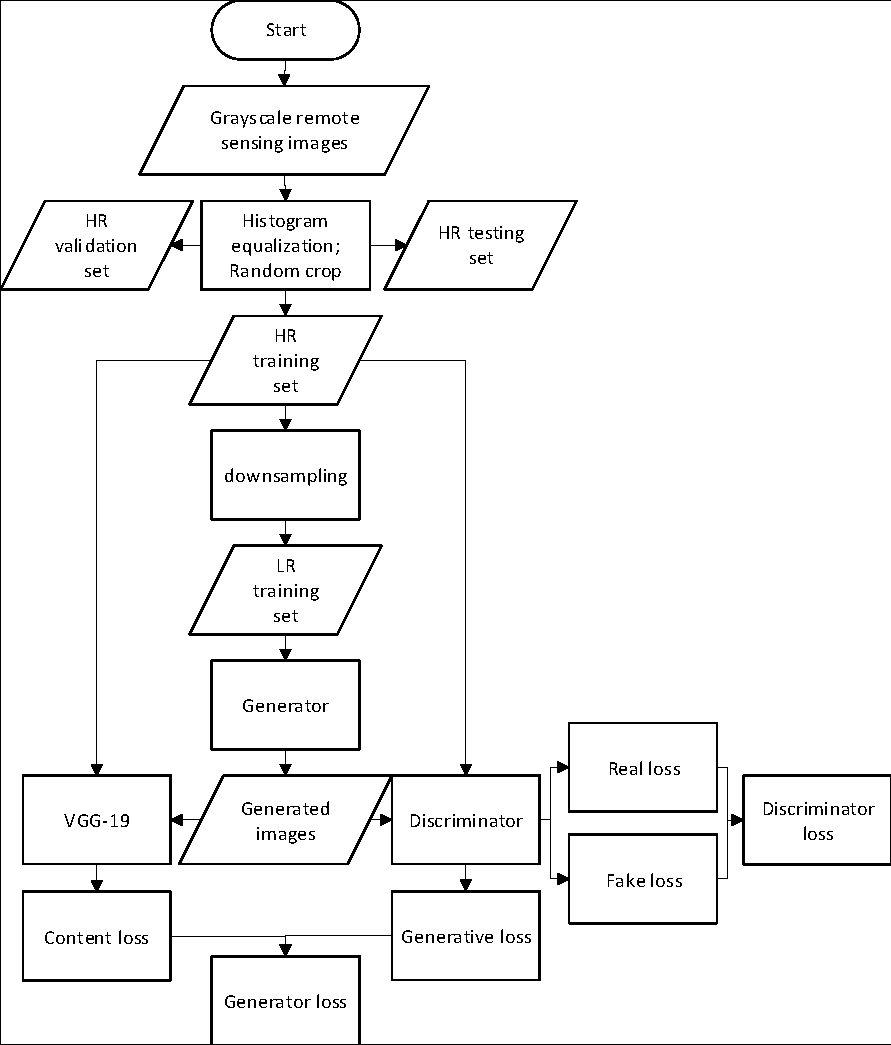
\includegraphics[width=0.8\textwidth]{fig1}
\end{center}
   \caption{Training flow chart of pbiSRGAN.}
\label{fig1}
\end{figure*}

 \begin{figure*}
\begin{center}
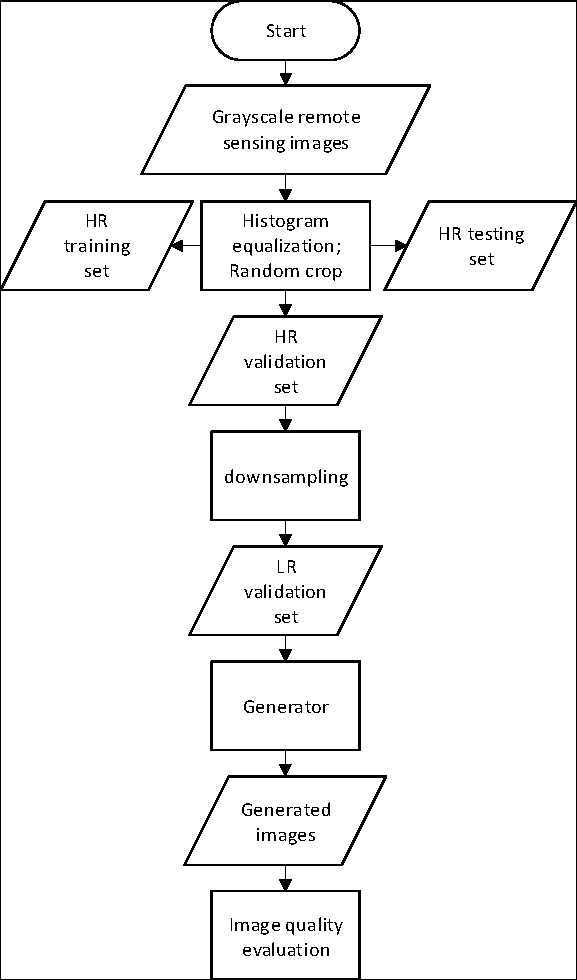
\includegraphics[width=0.5\textwidth]{fig2}
\end{center}
   \caption{Reconstructing flow chart of pbiSRGAN.}
\label{fig2}
\end{figure*}

 \begin{figure*}
\begin{center}
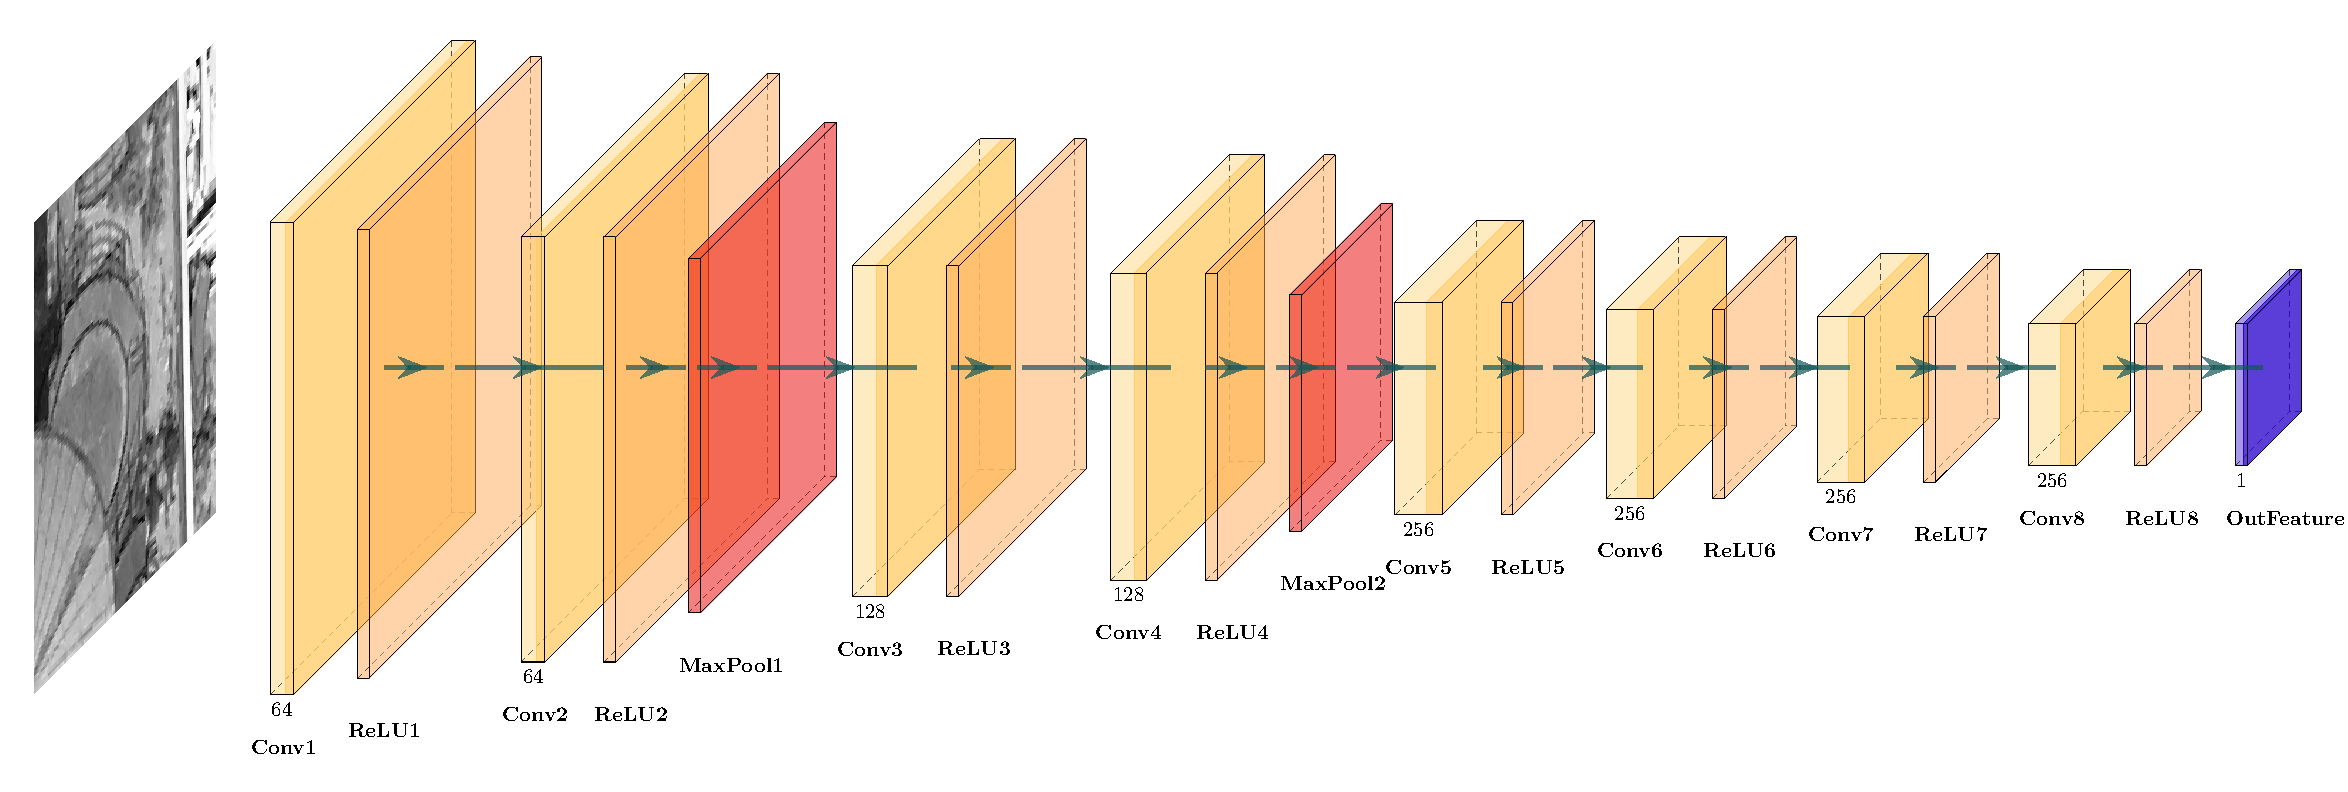
\includegraphics[width=1\textwidth]{fig3}
\end{center}
   \caption{Architecture of feature extractor network.}
\label{fig3}
\end{figure*}

 \begin{figure*}
\begin{center}
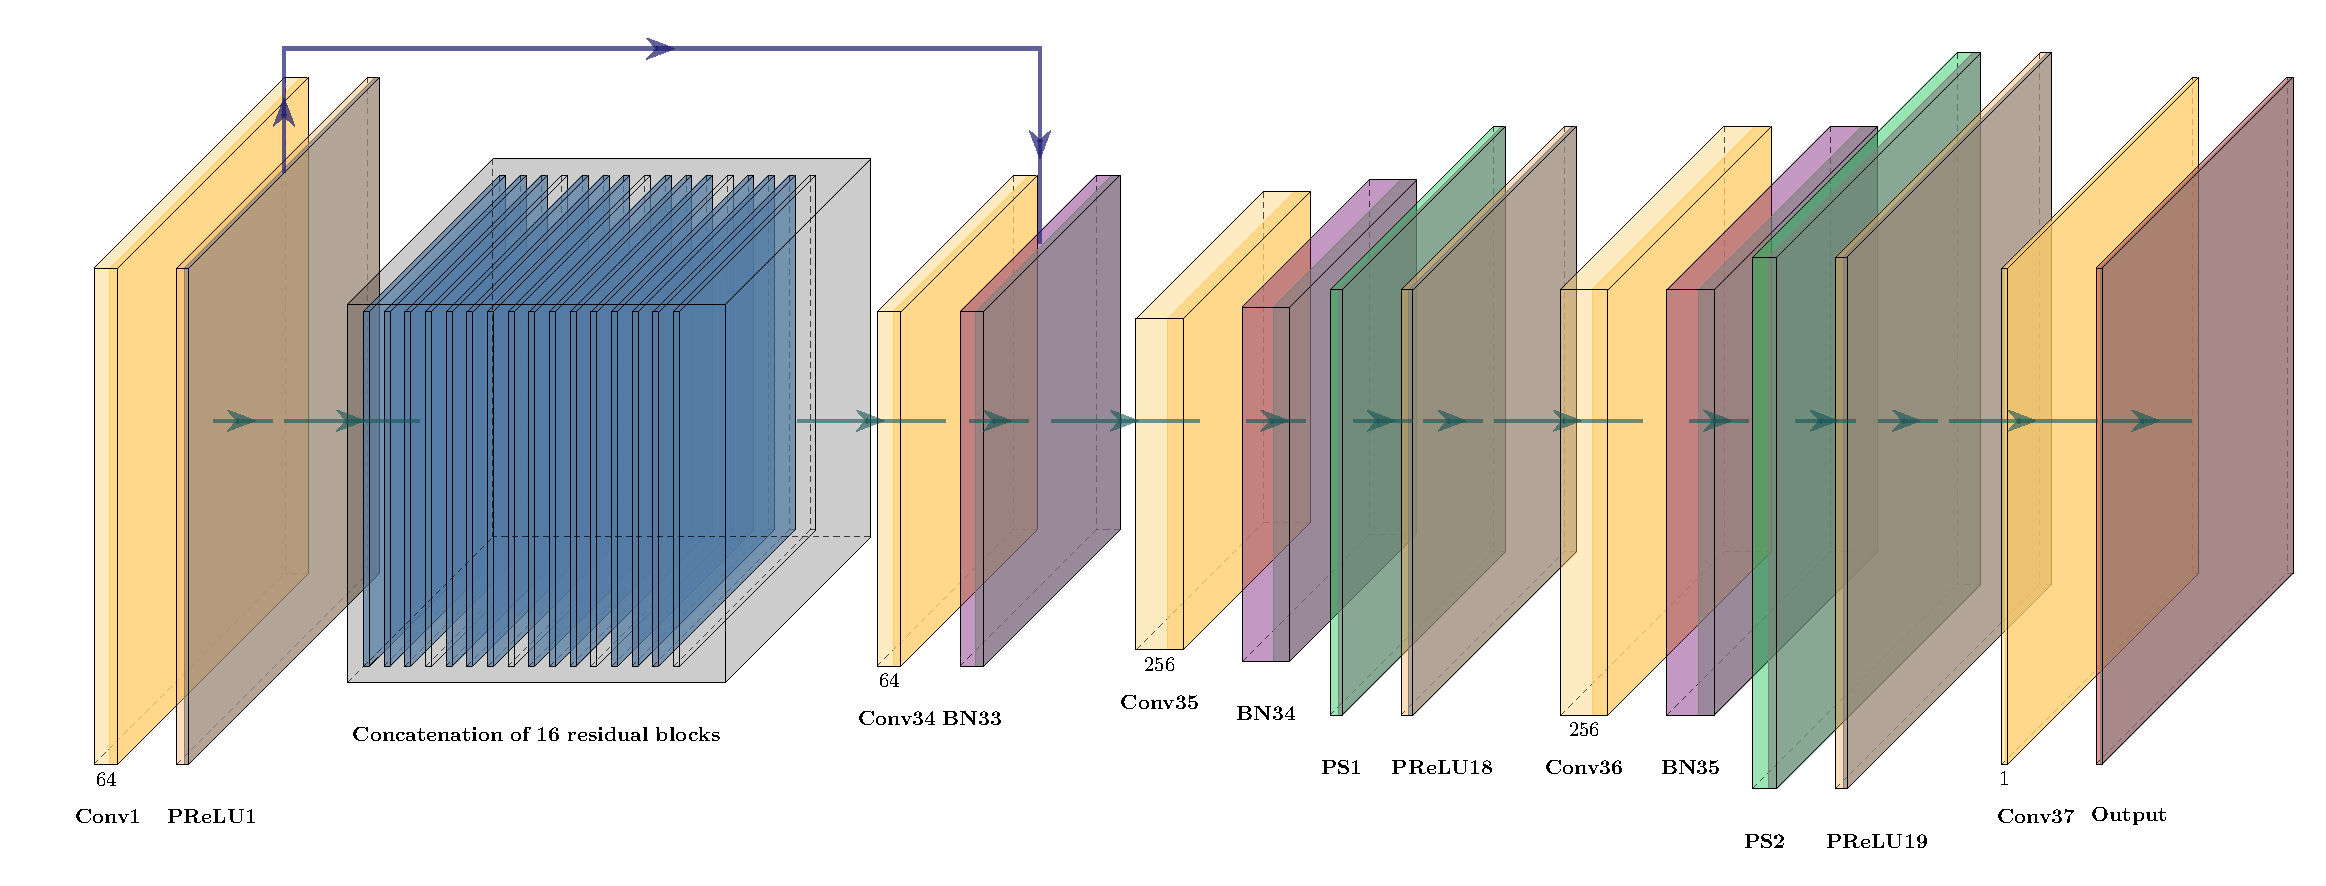
\includegraphics[width=1\textwidth]{fig4}
\end{center}
   \caption{Architecture of generative network.}
\label{fig4}
\end{figure*}

 \begin{figure*}
\begin{center}
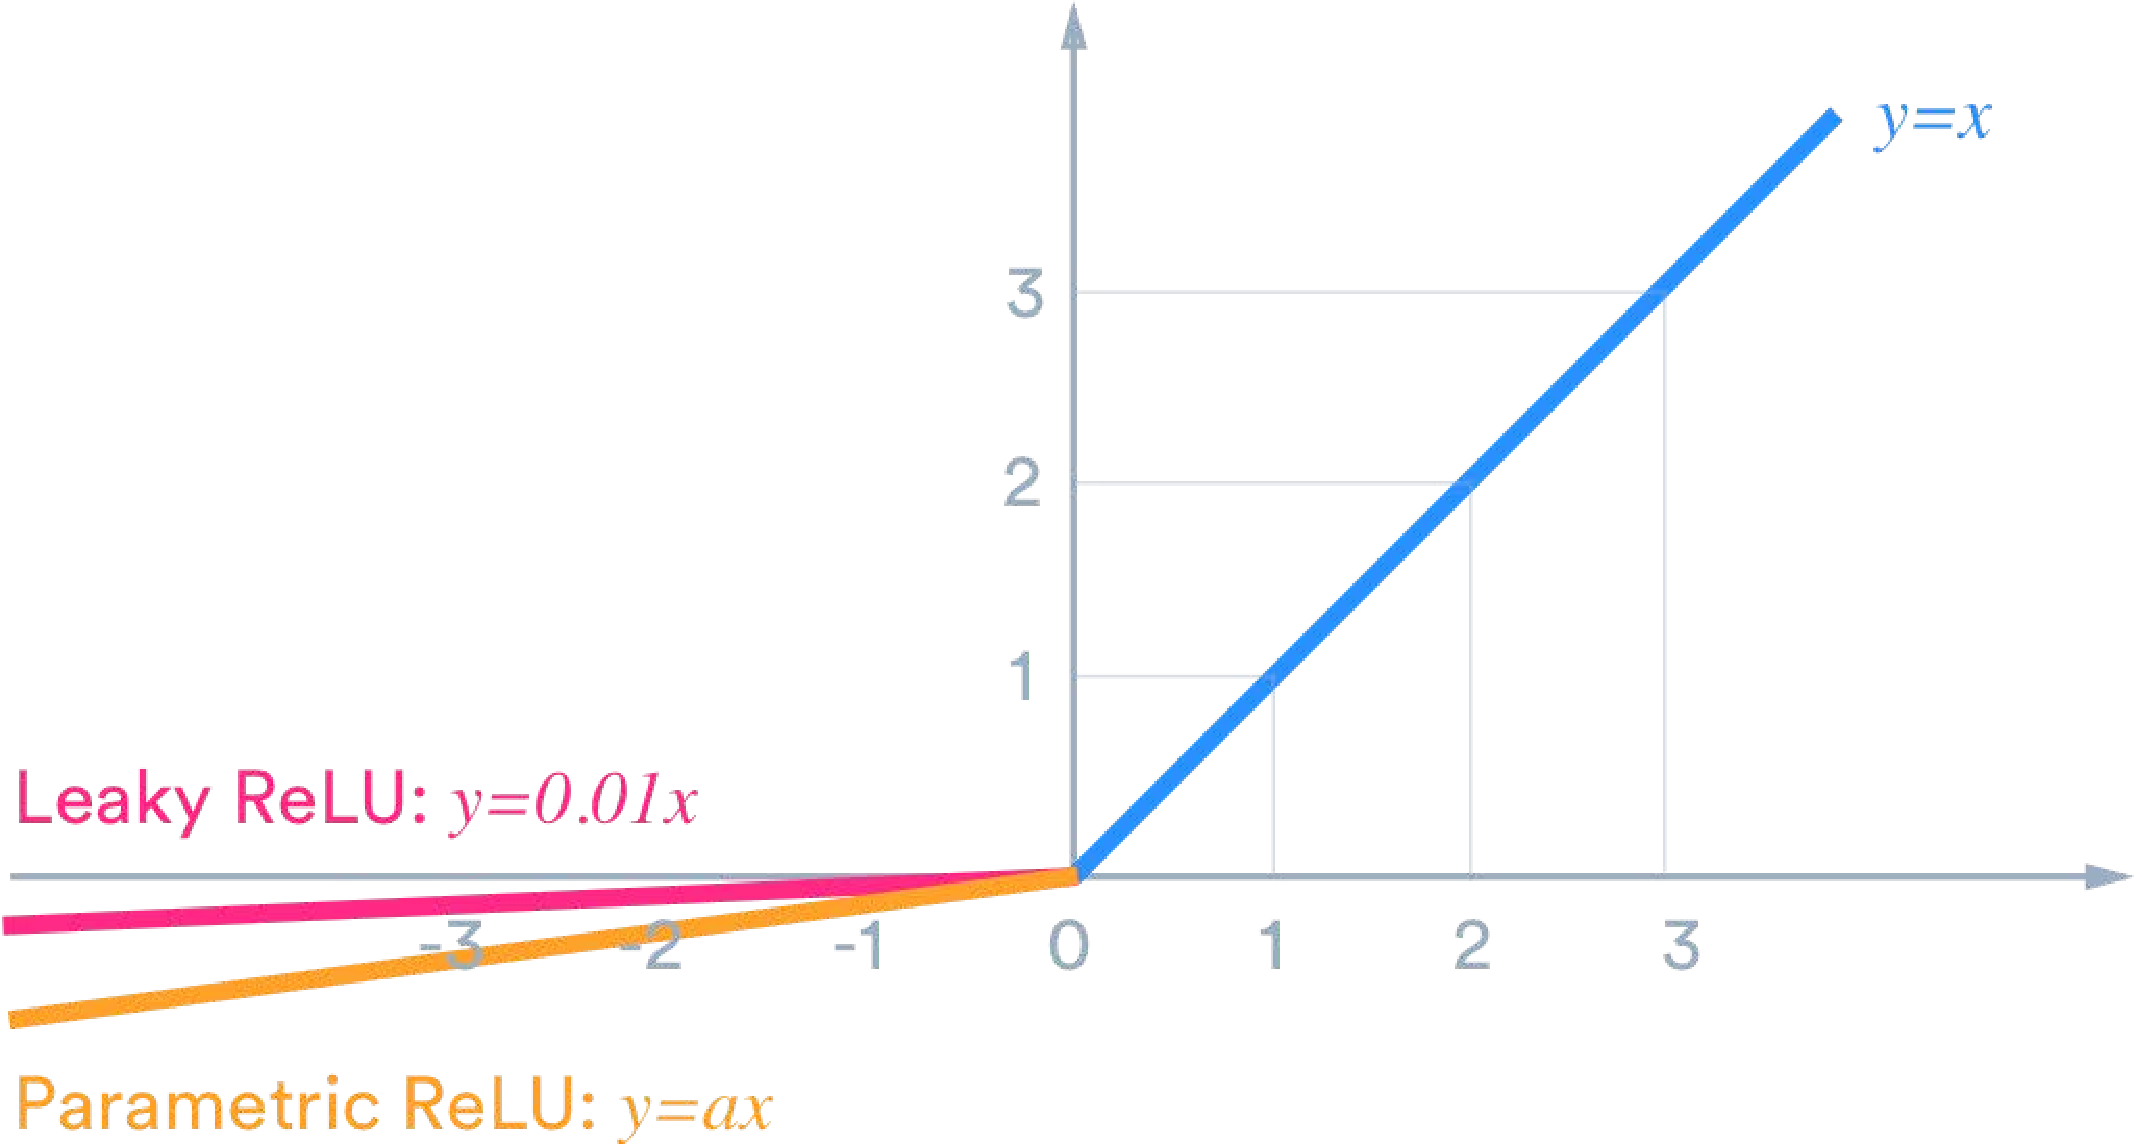
\includegraphics[width=1\textwidth]{fig5}
\end{center}
   \caption{Representation of LReLU and PReLU.}
\label{fig5}
\end{figure*}

 \begin{figure*}
\begin{center}
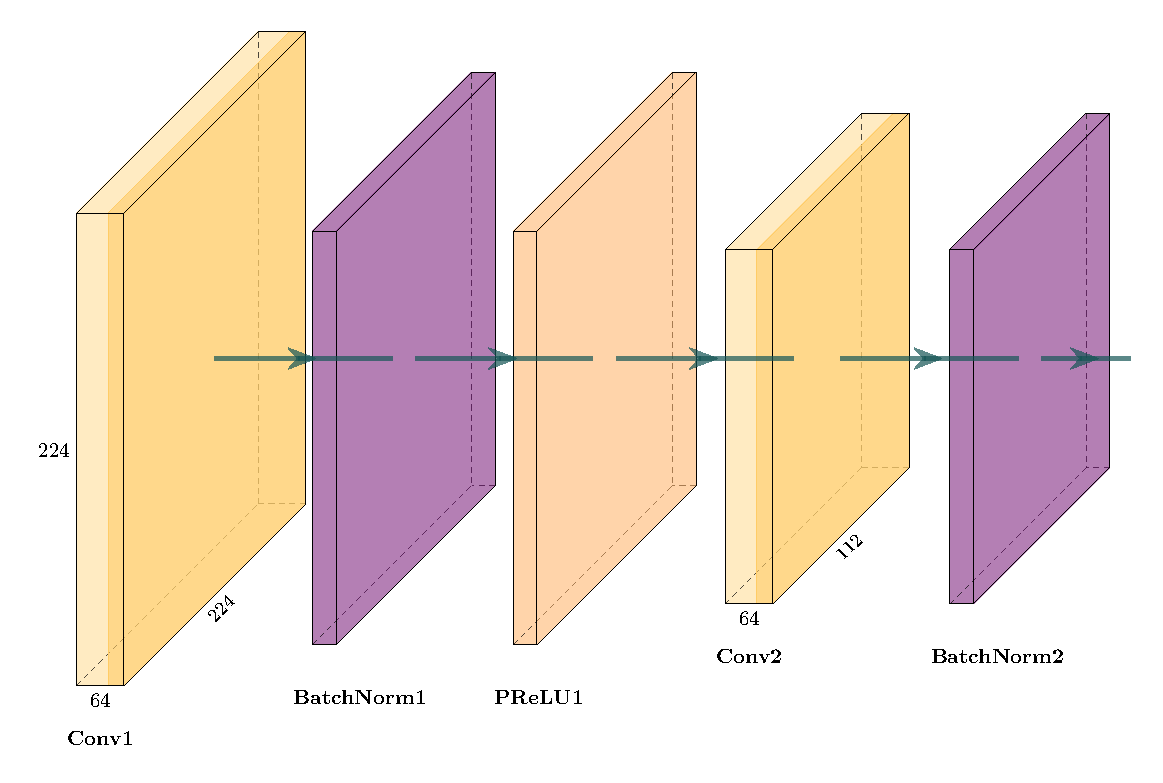
\includegraphics[width=1\textwidth]{fig6}
\end{center}
   \caption{Architecture of residual block.}
\label{fig6}
\end{figure*}

 \begin{figure*}
\begin{center}
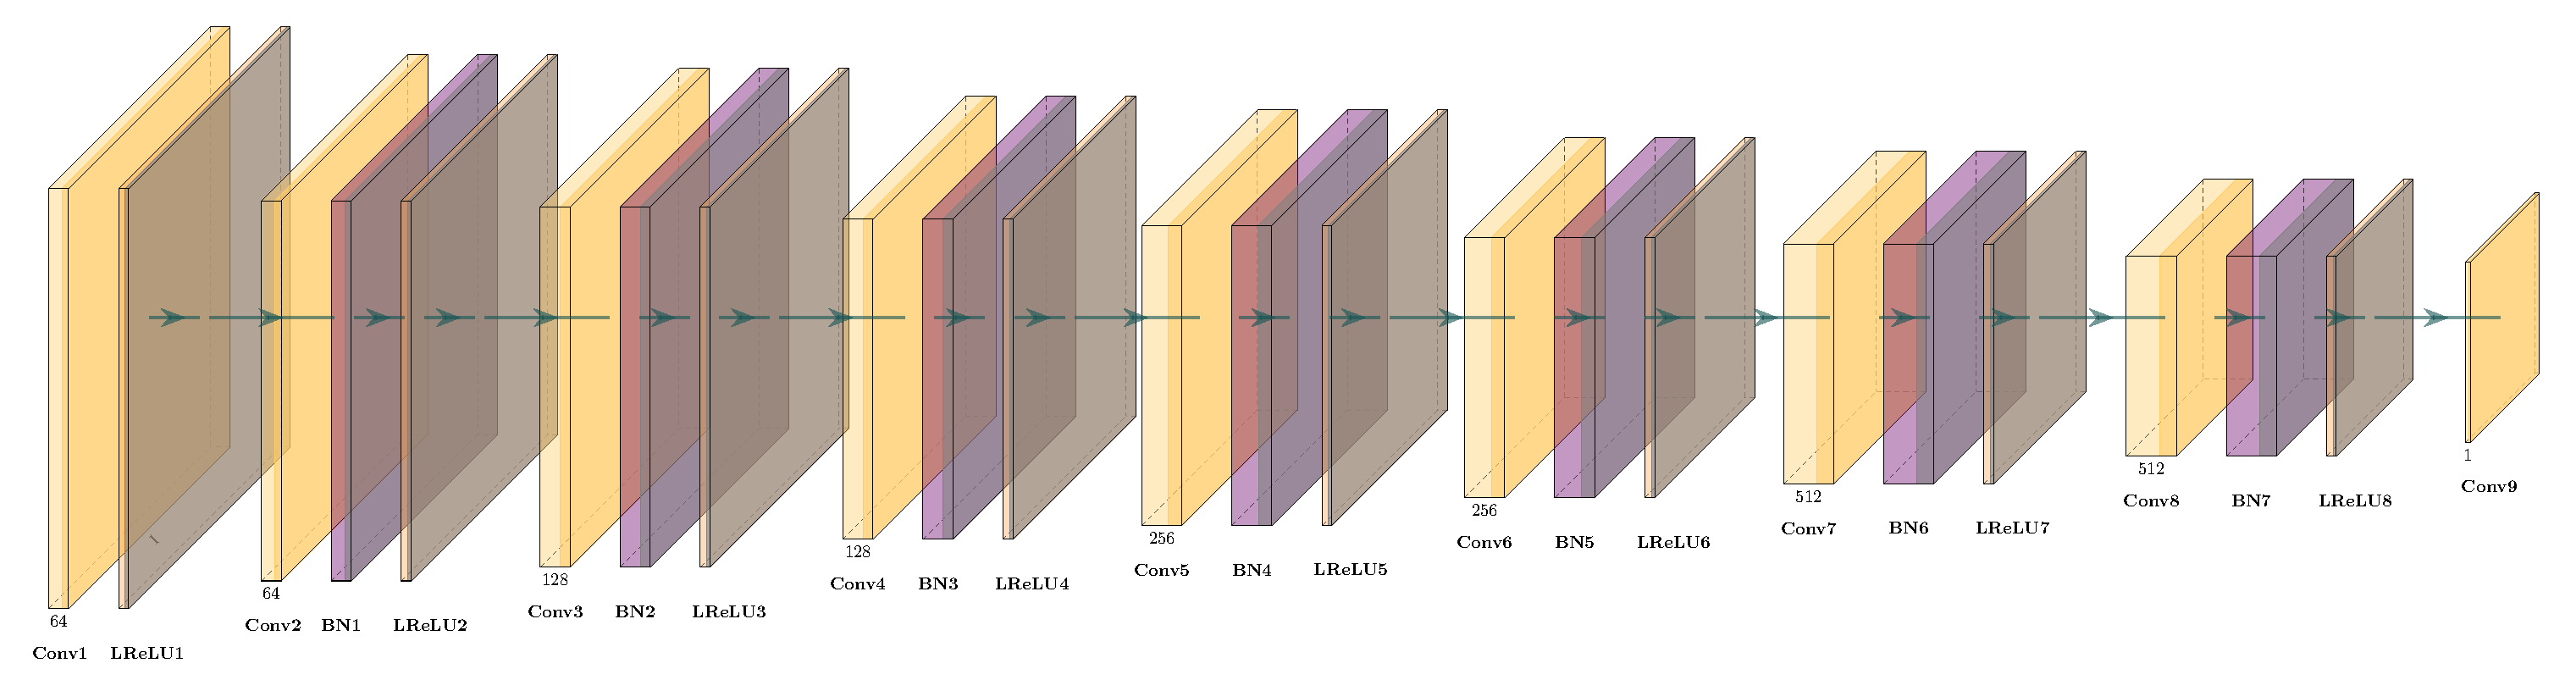
\includegraphics[width=1\textwidth]{fig7}
\end{center}
   \caption{Architecture of discriminator network.}
\label{fig7}
\end{figure*}

\begin{figure}%
\centering\begin{tabular}{c}
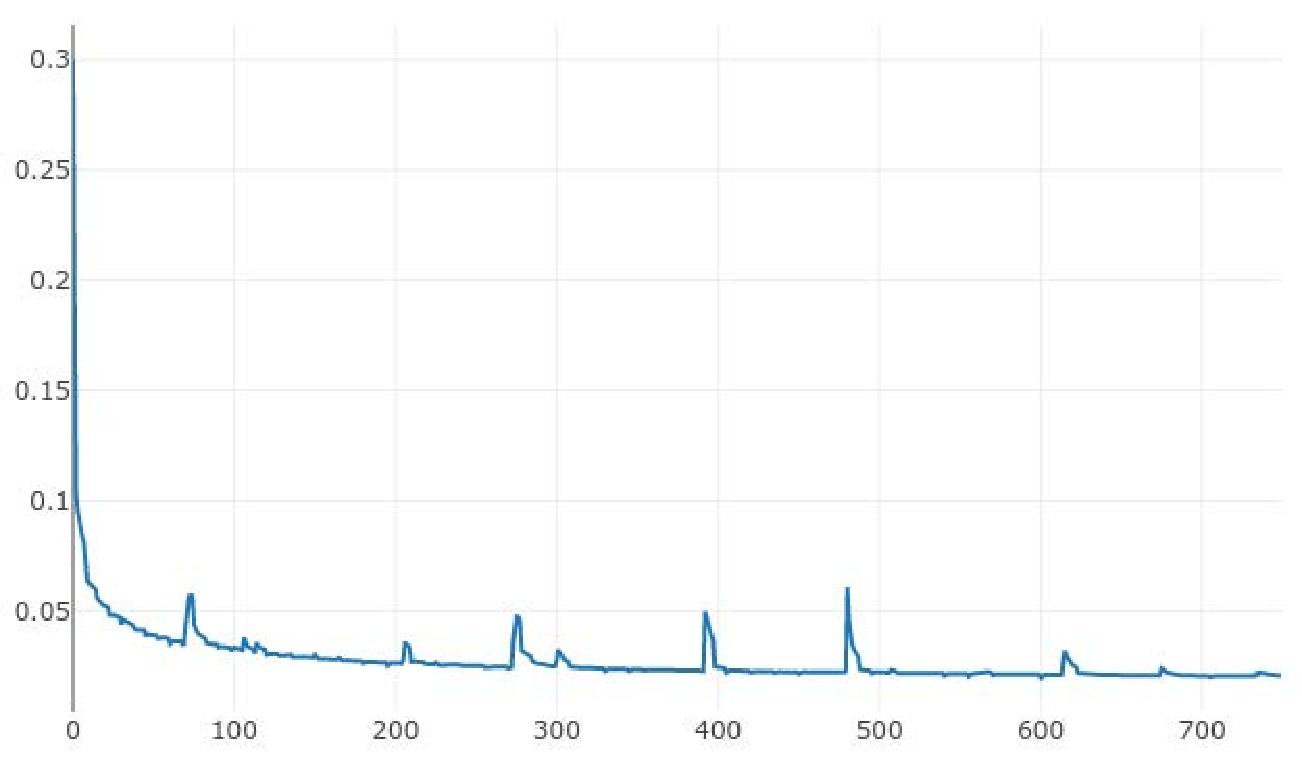
\includegraphics[width=0.5\textwidth]{fig8-a}\\
(a)\\[3ex]% add a little extra space
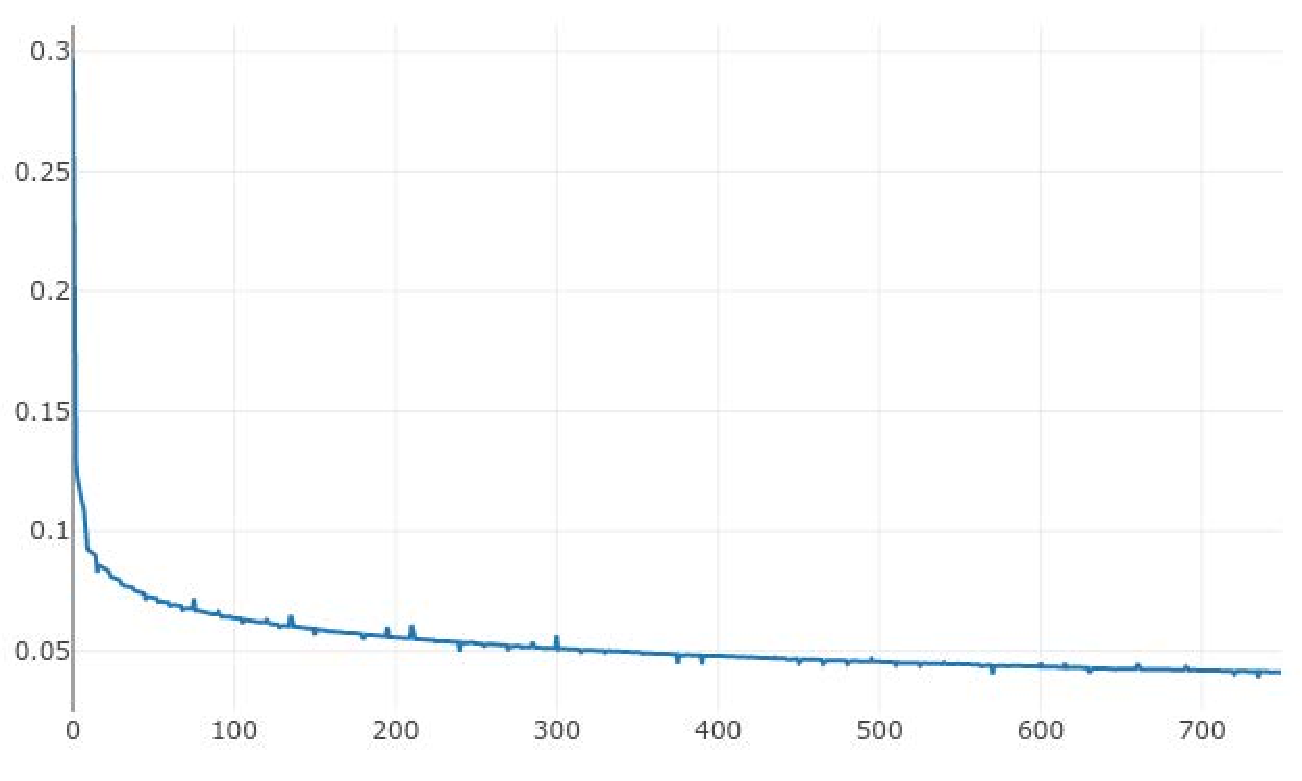
\includegraphics[width=0.5\textwidth]{fig8-b}\\
(b)\\[3ex]
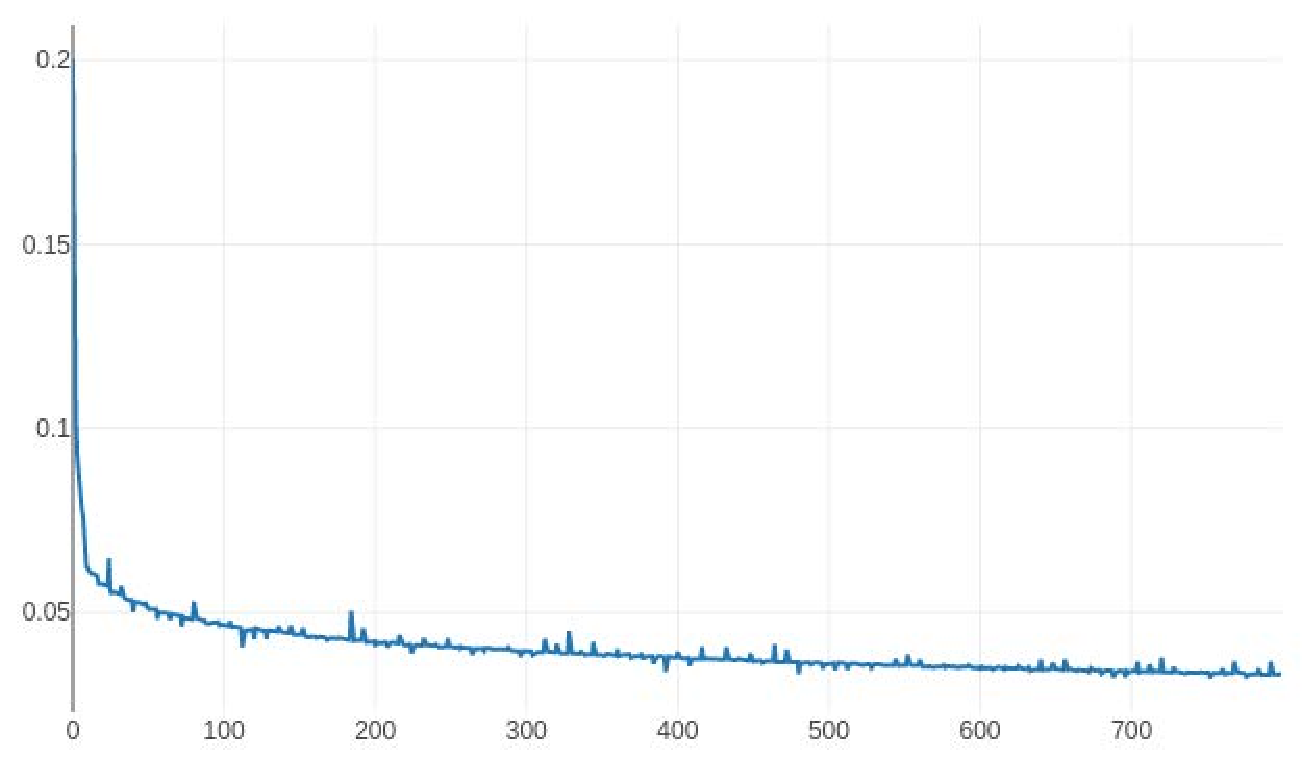
\includegraphics[width=0.5\textwidth]{fig8-c}\\
(c)
\end{tabular}
\caption{Batch con loss. (a) Group 1, (b) Group 2, (c) Group 3.}%
\label{fig8}%
\end{figure}

\begin{figure}%
\centering\begin{tabular}{c}
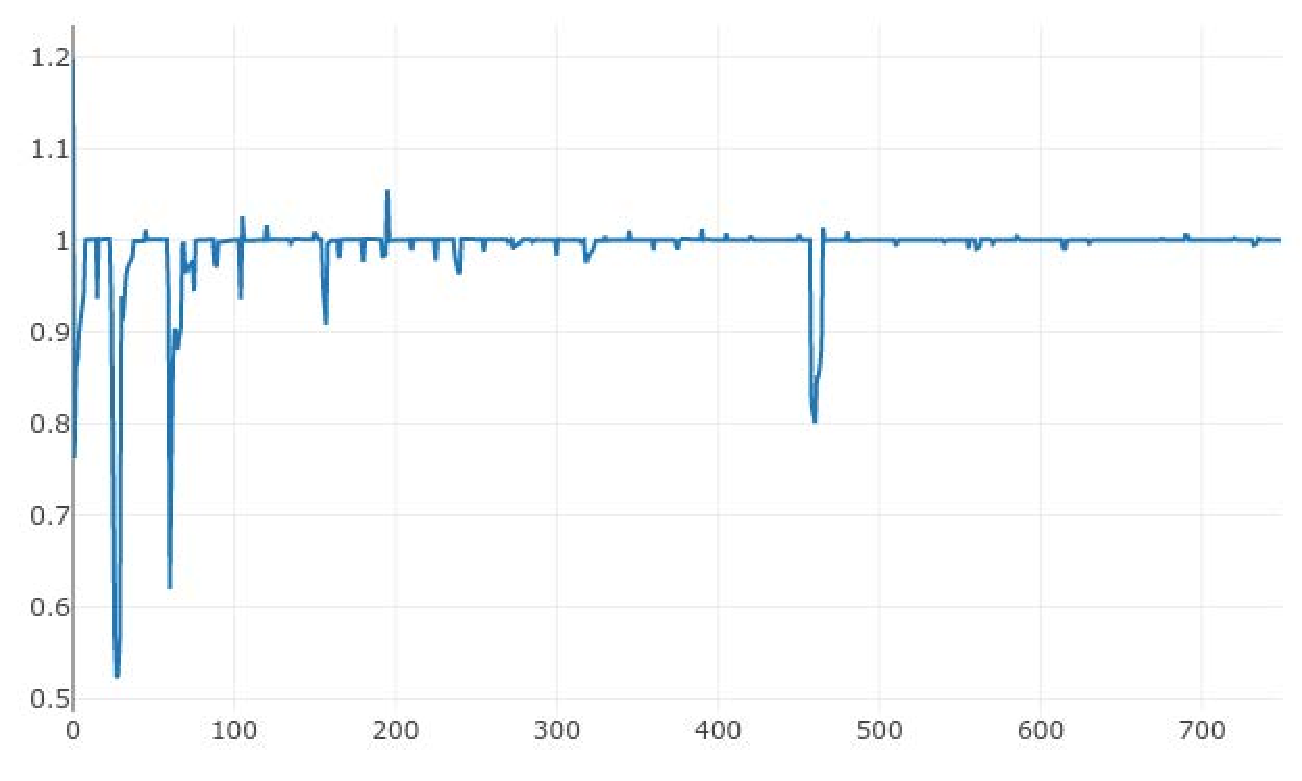
\includegraphics[width=0.5\textwidth]{fig9-a}\\
(a)\\[3ex]% add a little extra space
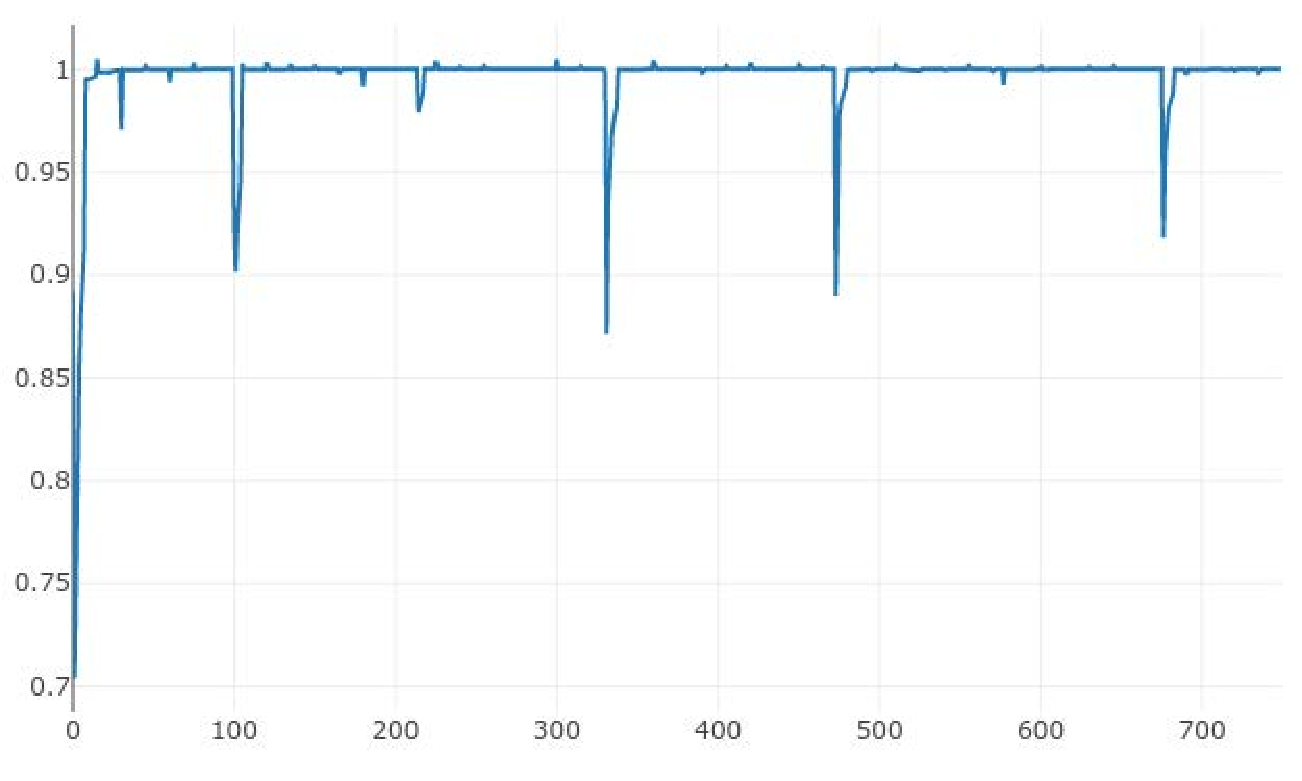
\includegraphics[width=0.5\textwidth]{fig9-b}\\
(b)\\[3ex]
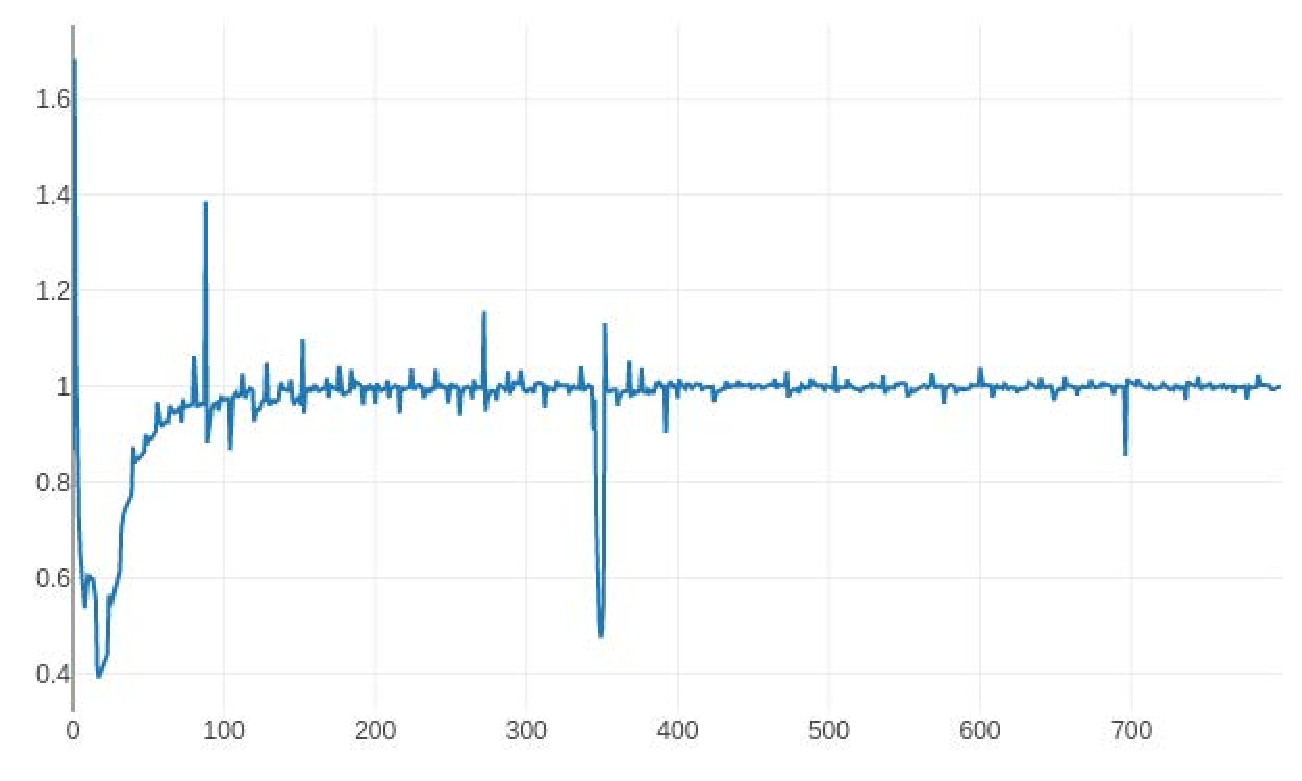
\includegraphics[width=0.5\textwidth]{fig9-c}\\
(c)
\end{tabular}
\caption{Batch gen los. (a) Group 1, (b) Group 2, (c) Group 3.}%
\label{fig9}%
\end{figure}

\begin{figure}%
\centering\begin{tabular}{c}
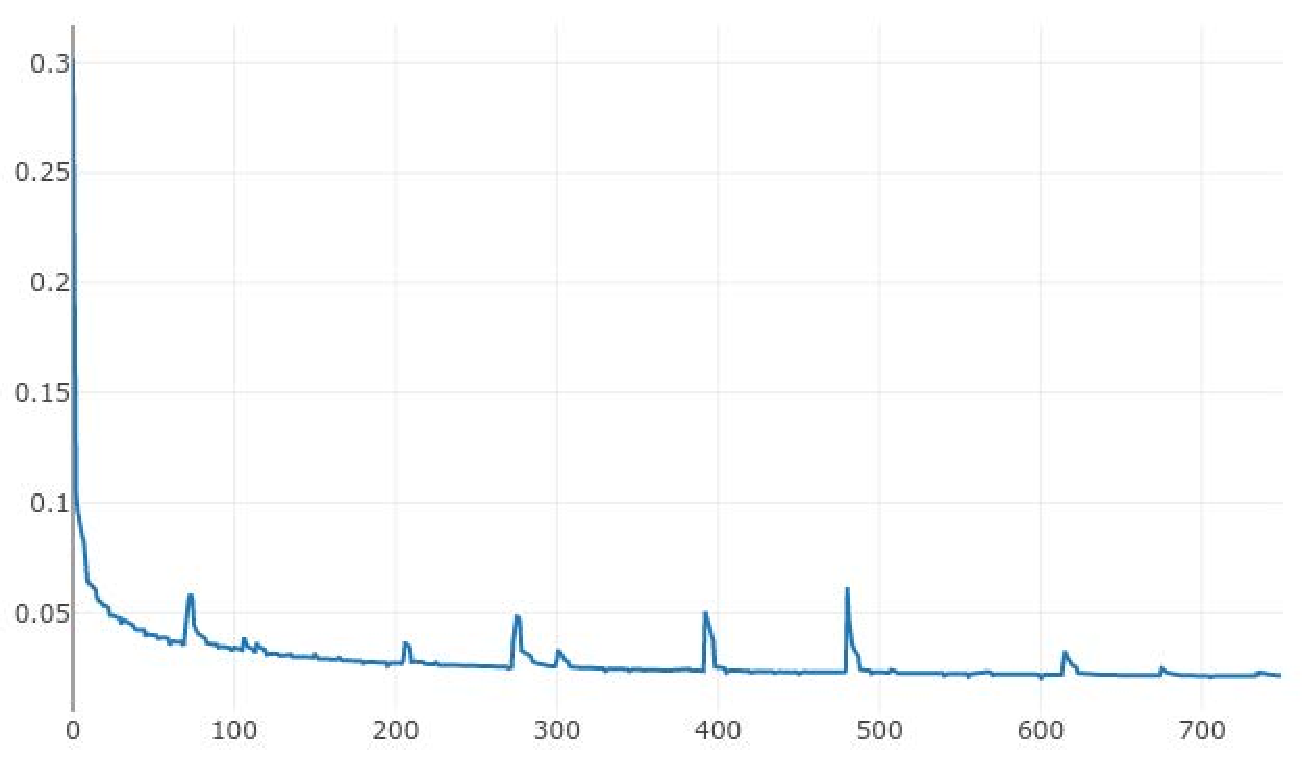
\includegraphics[width=0.5\textwidth]{fig10-a}\\
(a)\\[3ex]% add a little extra space
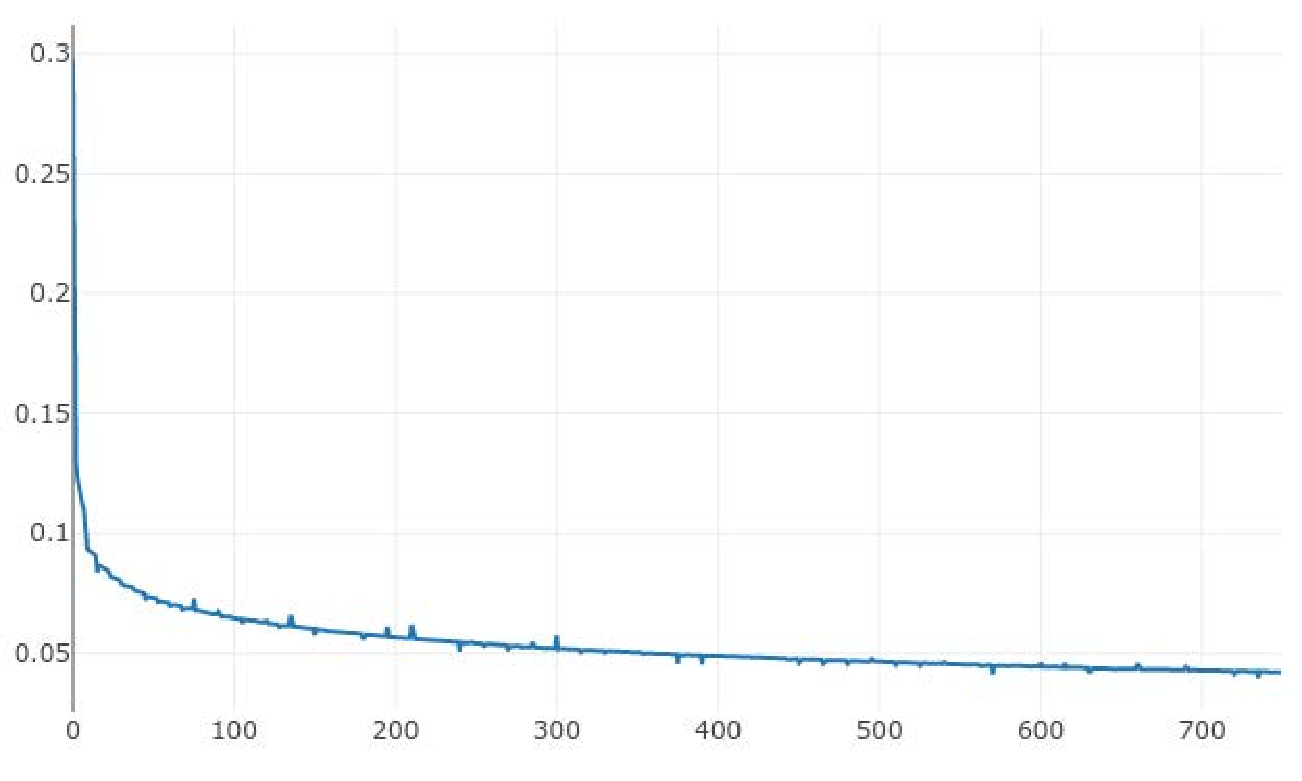
\includegraphics[width=0.5\textwidth]{fig10-b}\\
(b)\\[3ex]
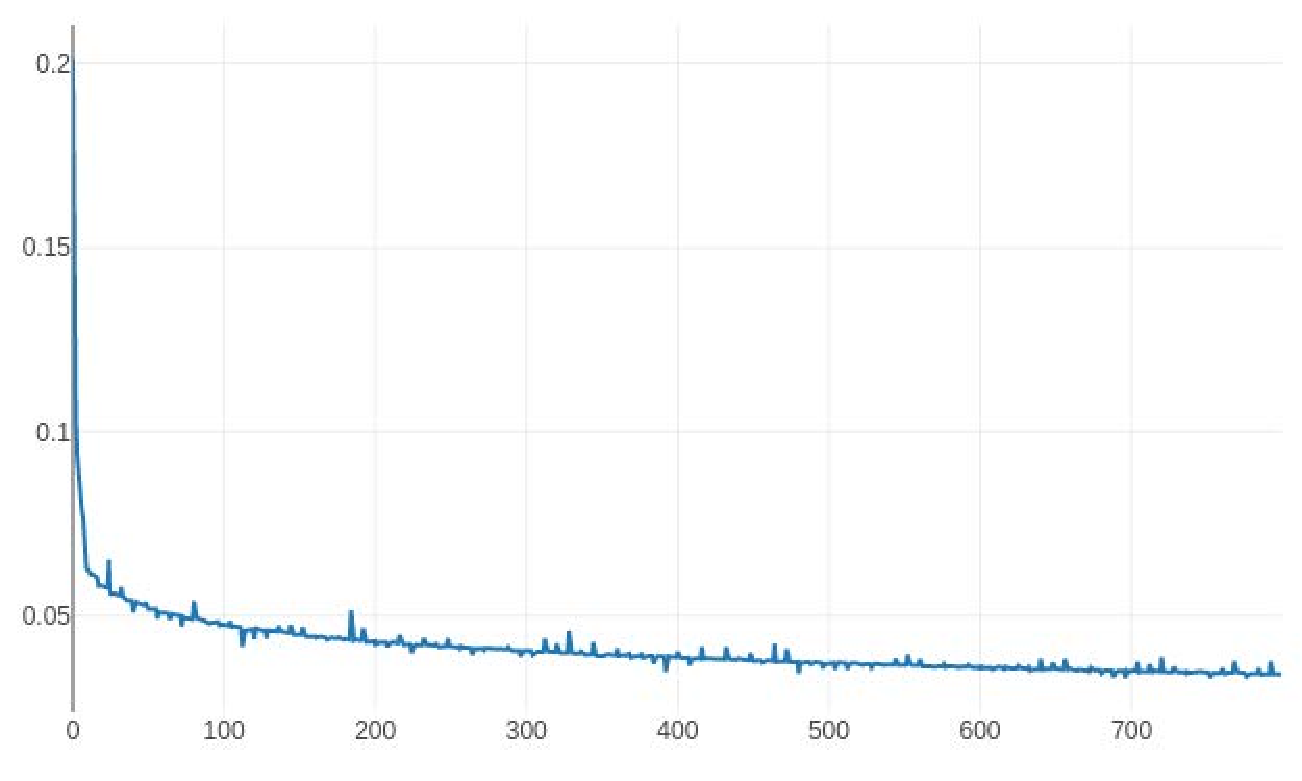
\includegraphics[width=0.5\textwidth]{fig10-c}\\
(c)
\end{tabular}
\caption{Batch G loss. (a) Group 1, (b) Group 2, (c) Group 3.}%
\label{fig10}%
\end{figure}

\begin{figure}%
\centering\begin{tabular}{c}
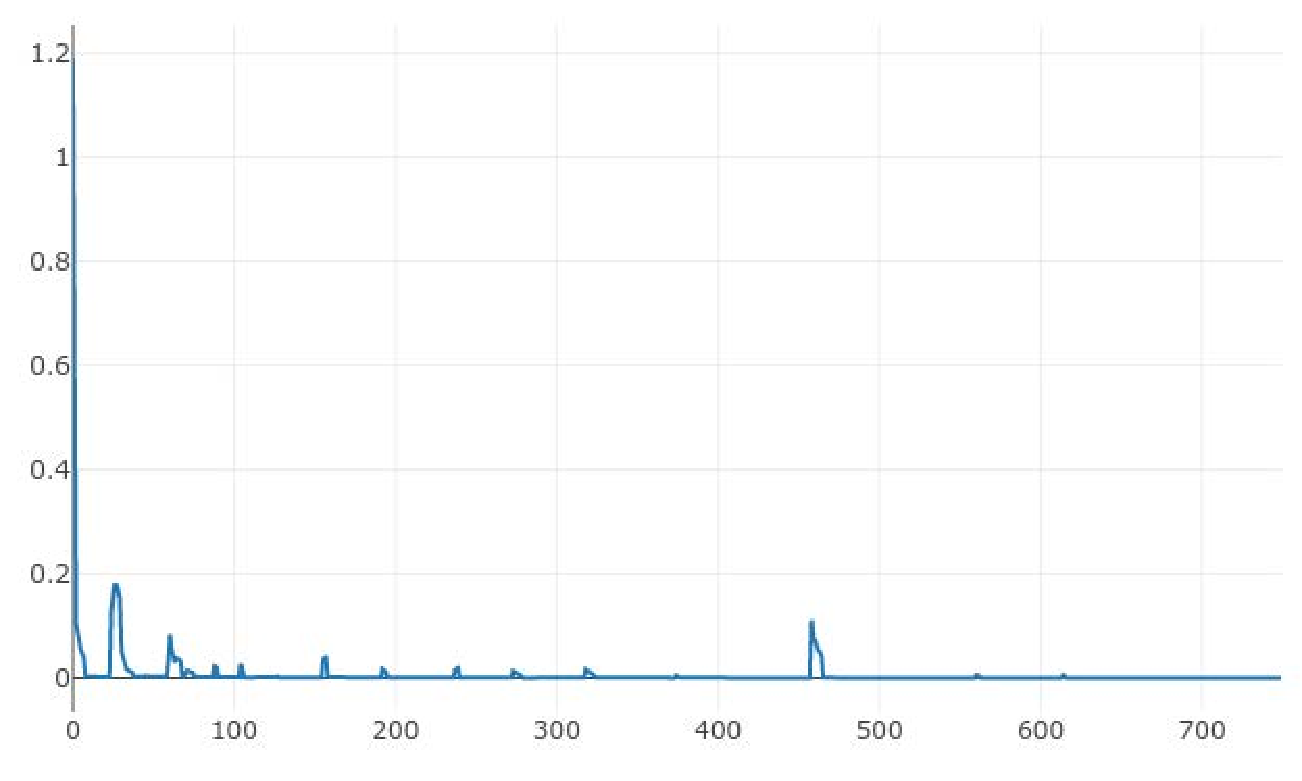
\includegraphics[width=0.5\textwidth]{fig11-a}\\
(a)\\[3ex]% add a little extra space
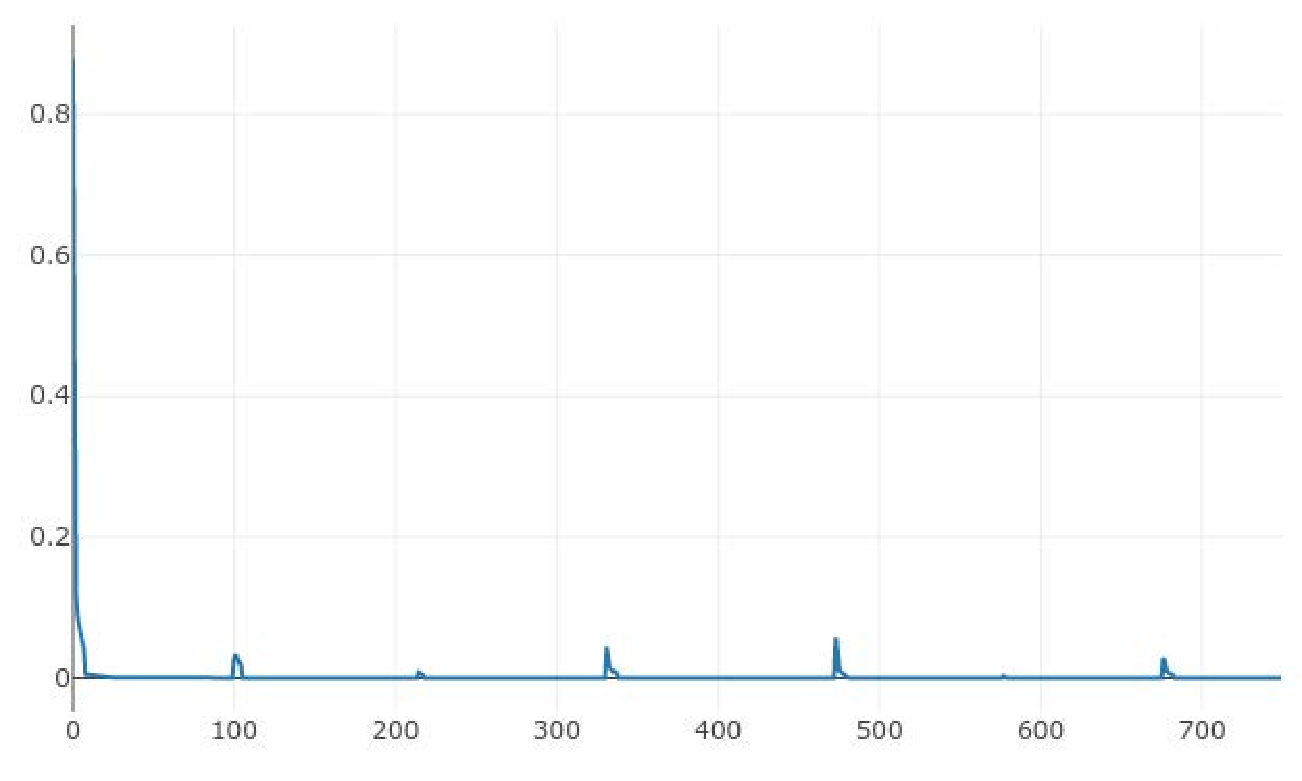
\includegraphics[width=0.5\textwidth]{fig11-b}\\
(b)\\[3ex]
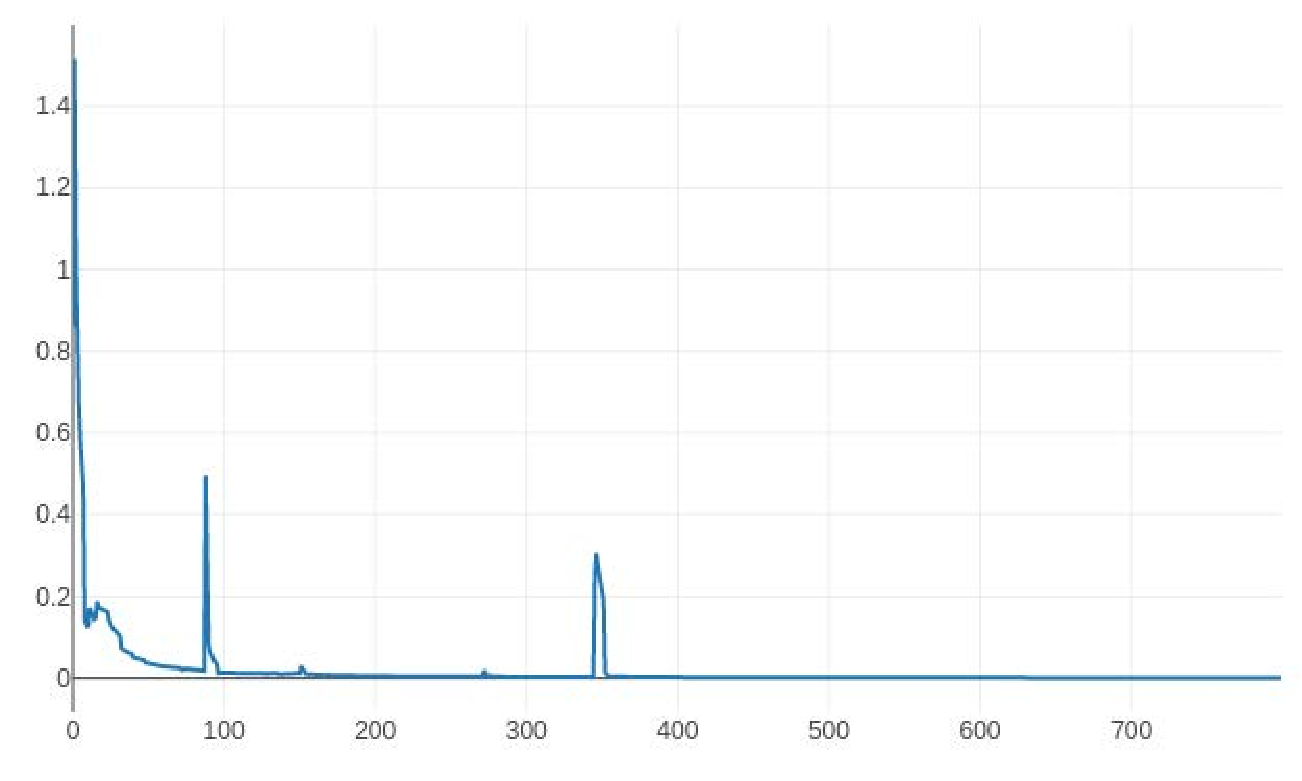
\includegraphics[width=0.5\textwidth]{fig11-c}\\
(c)
\end{tabular}
\caption{Batch real loss. (a) Group 1, (b) Group 2, (c) Group 3.}%
\label{fig11}%
\end{figure}

\begin{figure}%
\centering\begin{tabular}{c}
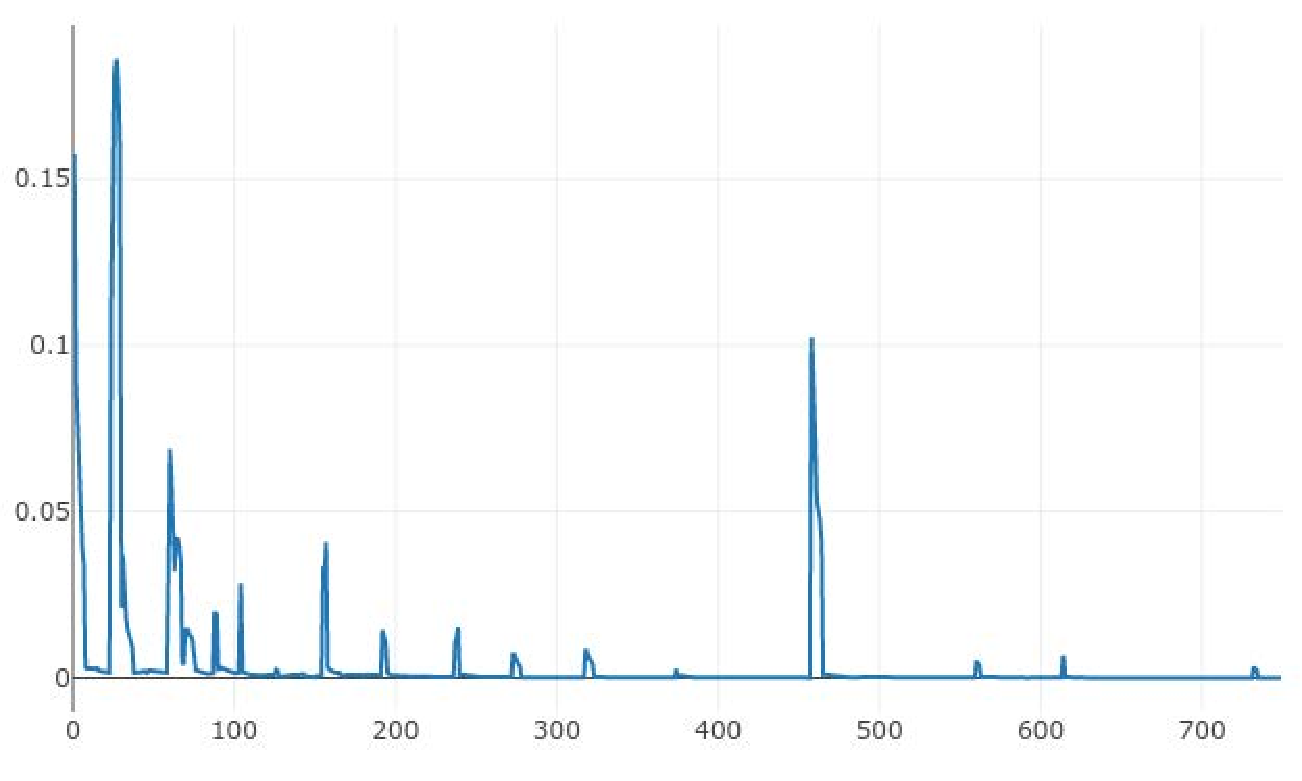
\includegraphics[width=0.5\textwidth]{fig12-a}\\
(a)\\[3ex]% add a little extra space
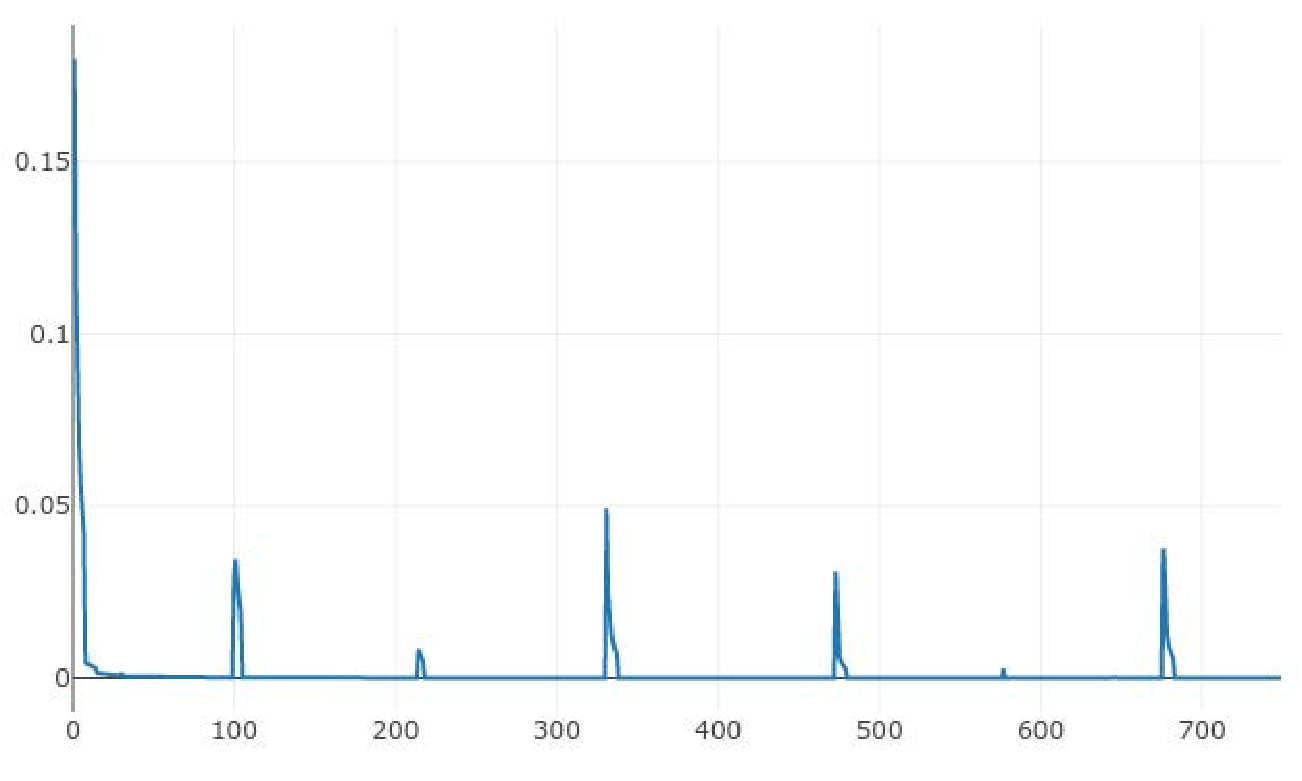
\includegraphics[width=0.5\textwidth]{fig12-b}\\
(b)\\[3ex]
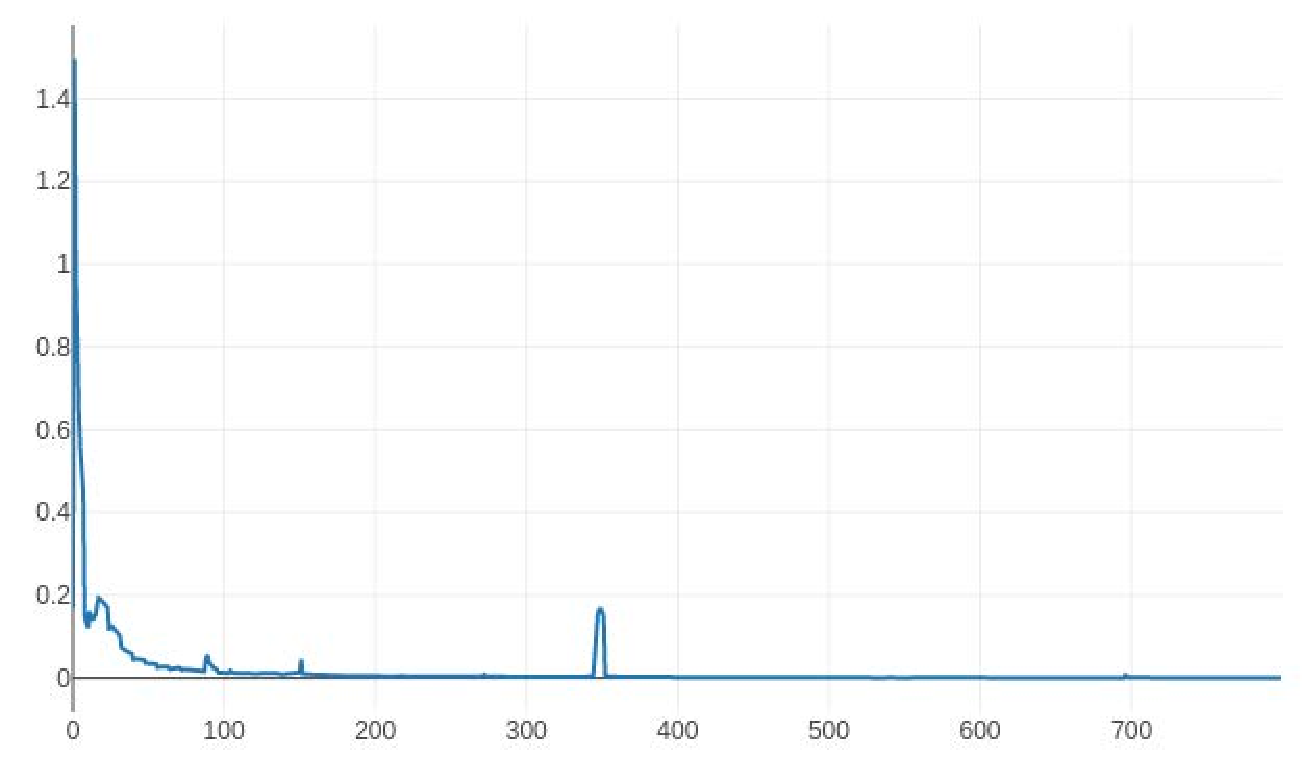
\includegraphics[width=0.5\textwidth]{fig12-c}\\
(c)
\end{tabular}
\caption{Batch fake loss. (a) Group 1, (b) Group 2, (c) Group 3.}%
\label{fig12}%
\end{figure}

\begin{figure}%
\centering\begin{tabular}{c}
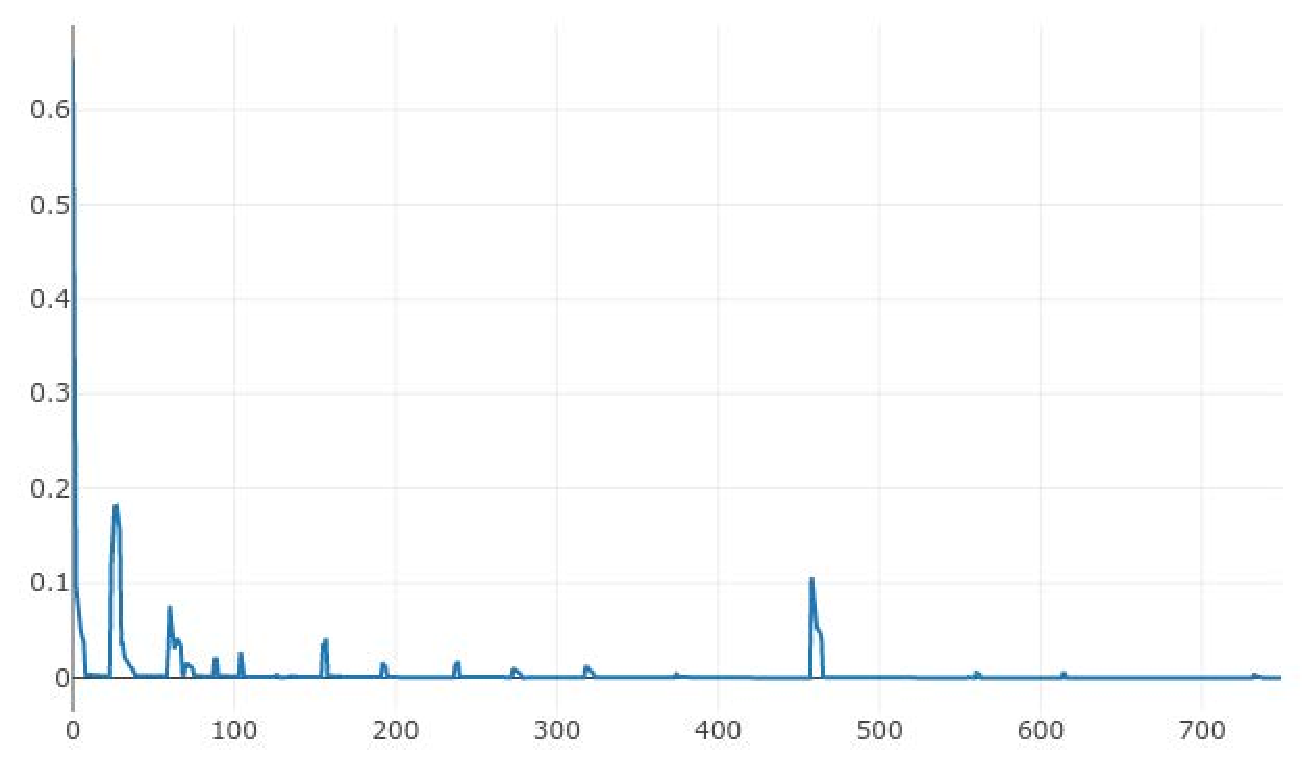
\includegraphics[width=0.5\textwidth]{fig13-a}\\
(a)\\[3ex]% add a little extra space
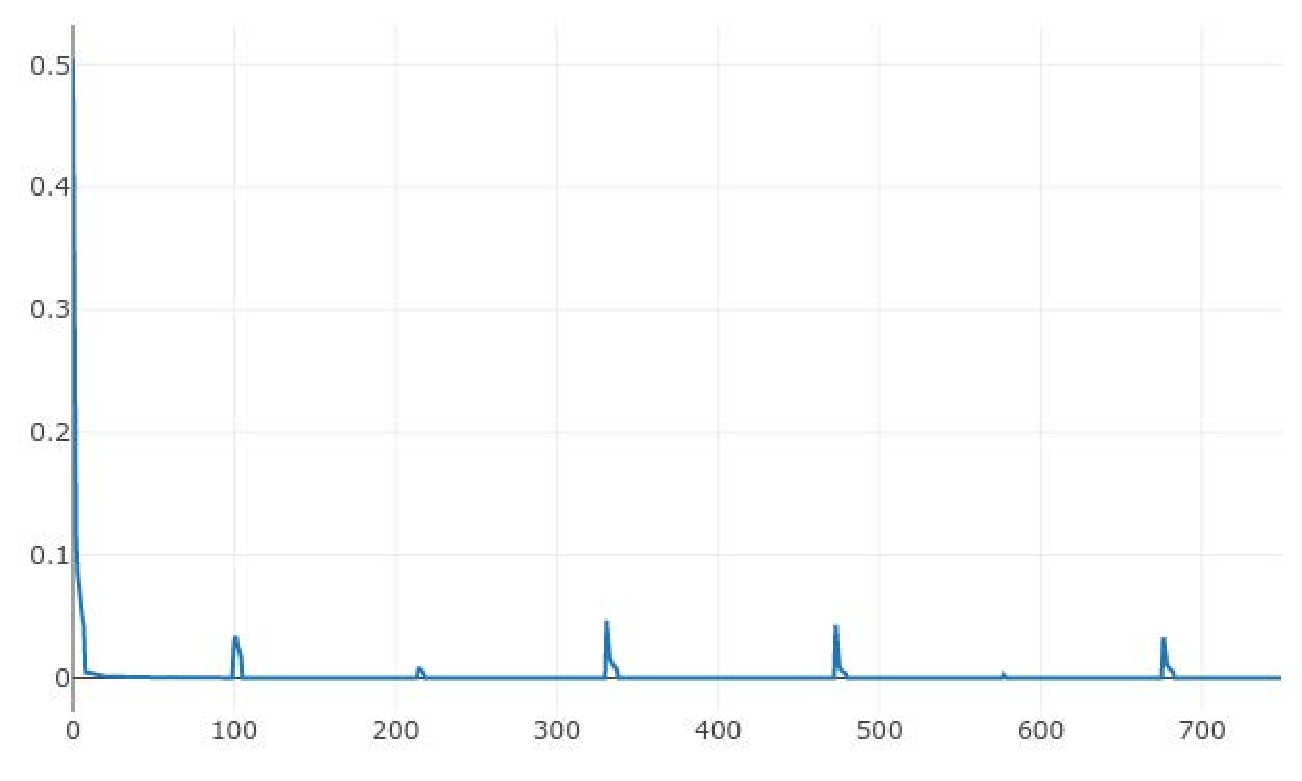
\includegraphics[width=0.5\textwidth]{fig13-b}\\
(b)\\[3ex]
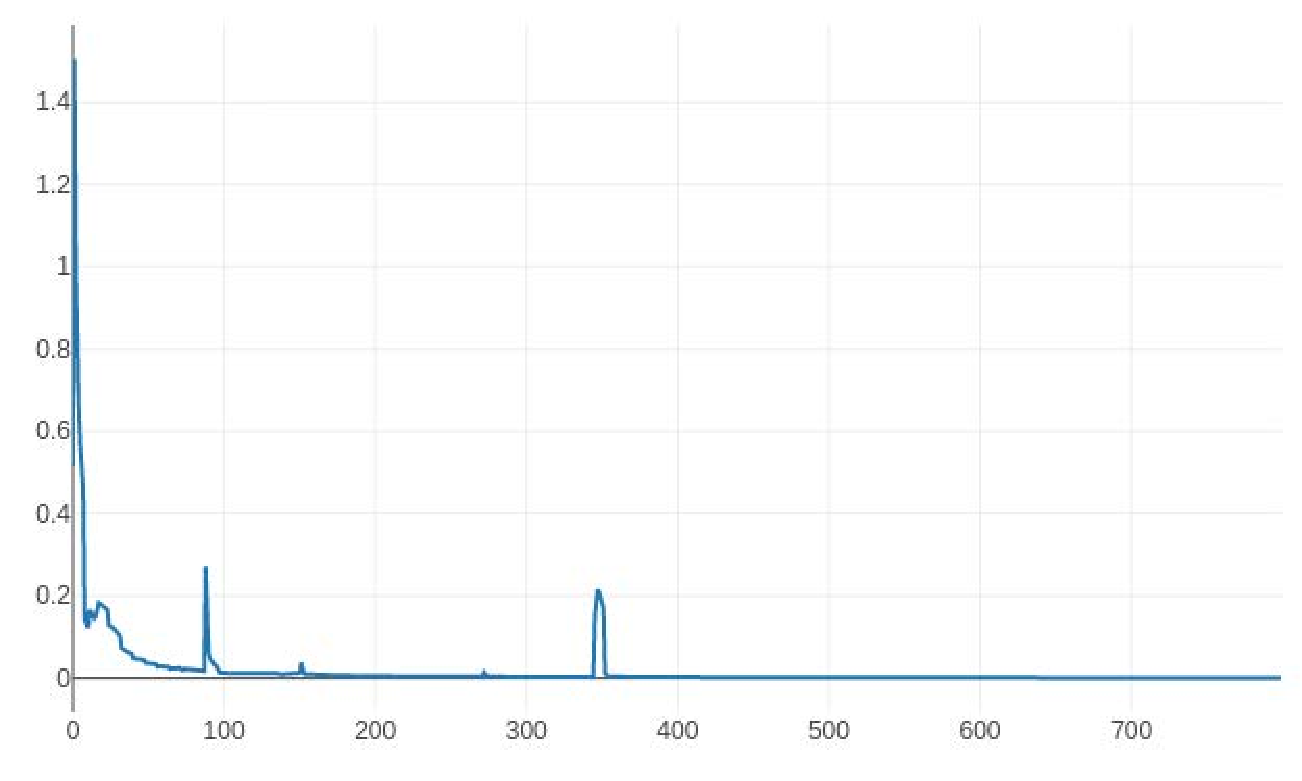
\includegraphics[width=0.5\textwidth]{fig13-c}\\
(c)
\end{tabular}
\caption{Batch D loss. (a) Group 1, (b) Group 2, (c) Group 3.}%
\label{fig13}%
\end{figure}

\begin{figure}%
\centering\begin{tabular}{c}
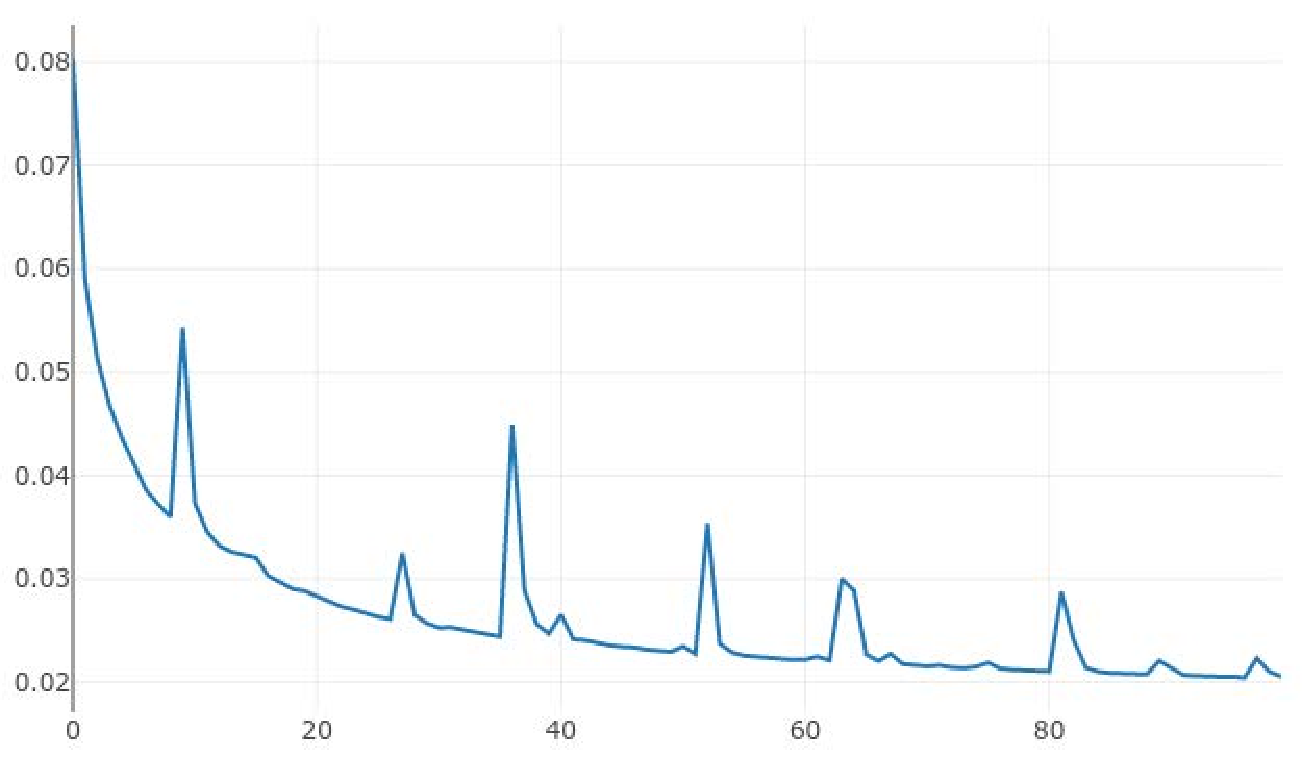
\includegraphics[width=0.5\textwidth]{fig14-a}\\
(a)\\[3ex]% add a little extra space
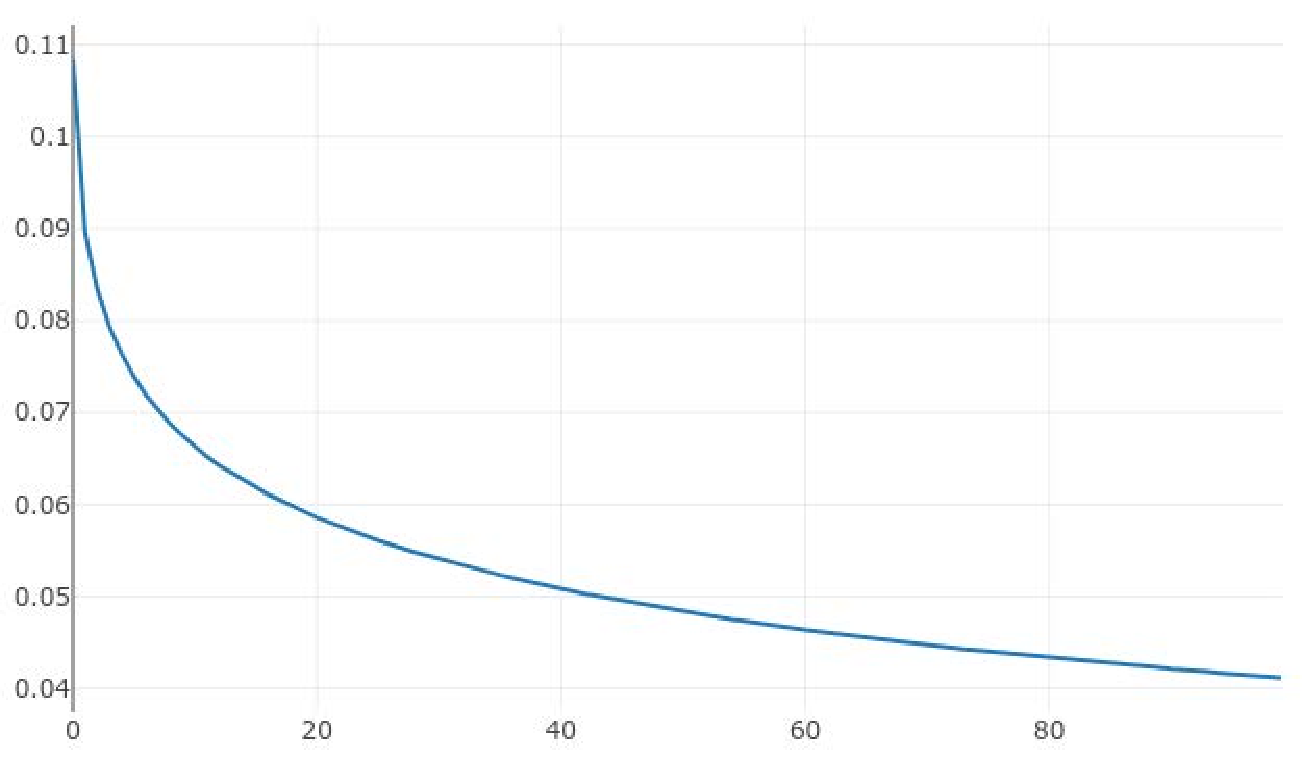
\includegraphics[width=0.5\textwidth]{fig14-b}\\
(b)\\[3ex]
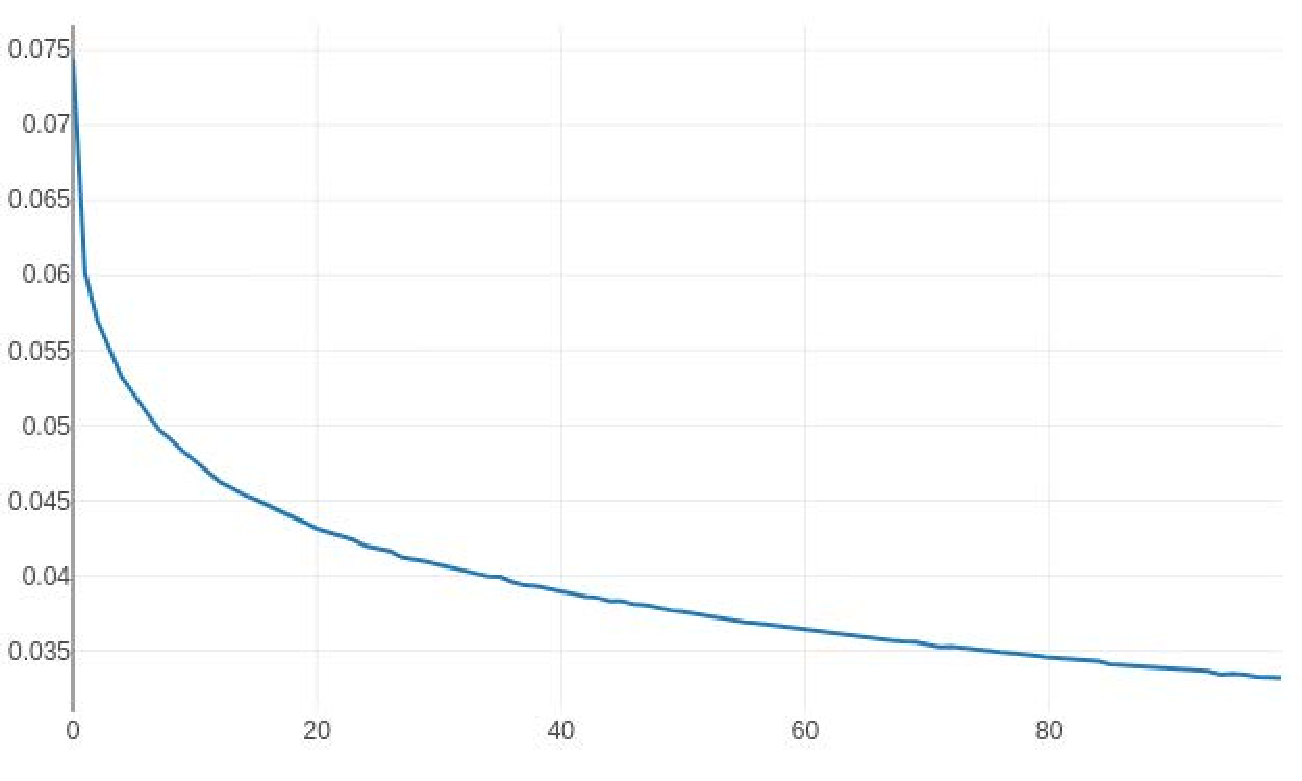
\includegraphics[width=0.5\textwidth]{fig14-c}\\
(c)
\end{tabular}
\caption{Epoch con loss. (a) Group 1, (b) Group 2, (c) Group 3.}%
\label{fig14}%
\end{figure}

\begin{figure}%
\centering\begin{tabular}{c}
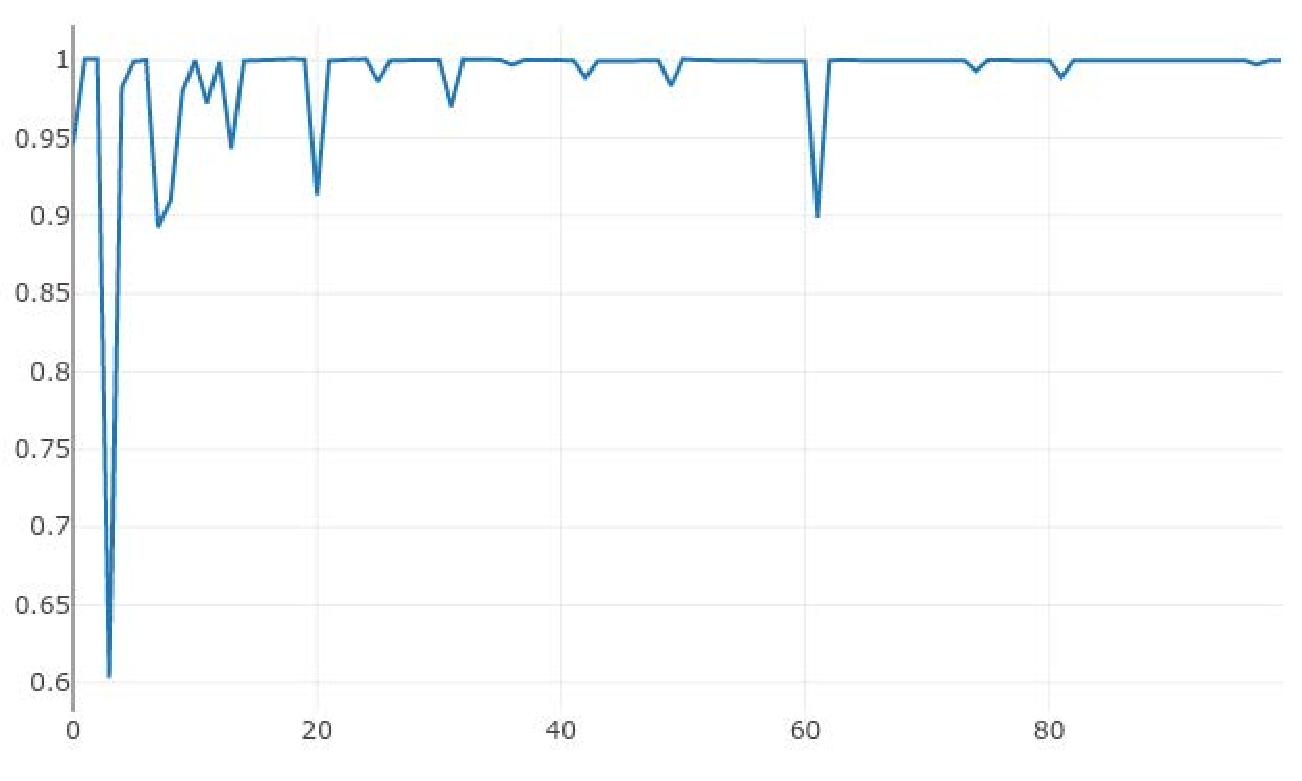
\includegraphics[width=0.5\textwidth]{fig15-a}\\
(a)\\[3ex]% add a little extra space
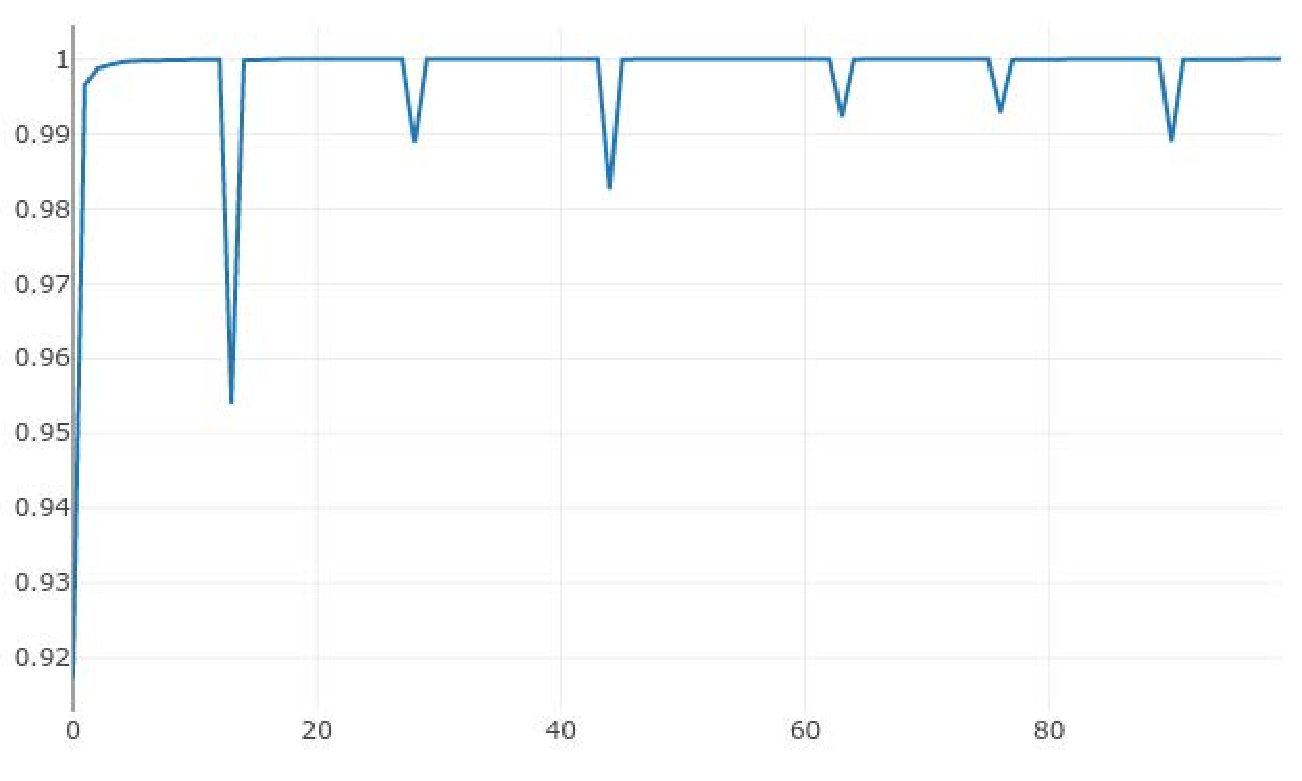
\includegraphics[width=0.5\textwidth]{fig15-b}\\
(b)\\[3ex]
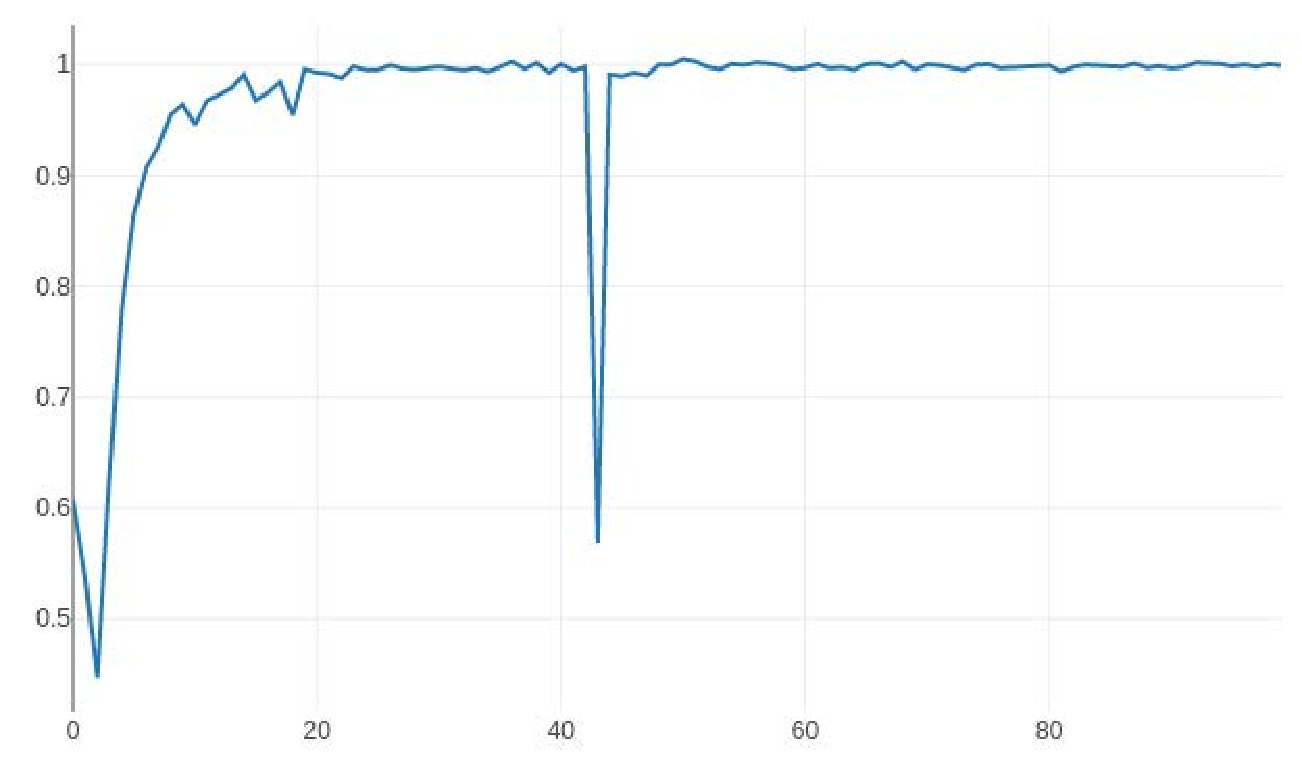
\includegraphics[width=0.5\textwidth]{fig15-c}\\
(c)
\end{tabular}
\caption{Epoch gen loss. (a) Group 1, (b) Group 2, (c) Group 3.}%
\label{fig15}%
\end{figure}

\begin{figure}%
\centering\begin{tabular}{c}
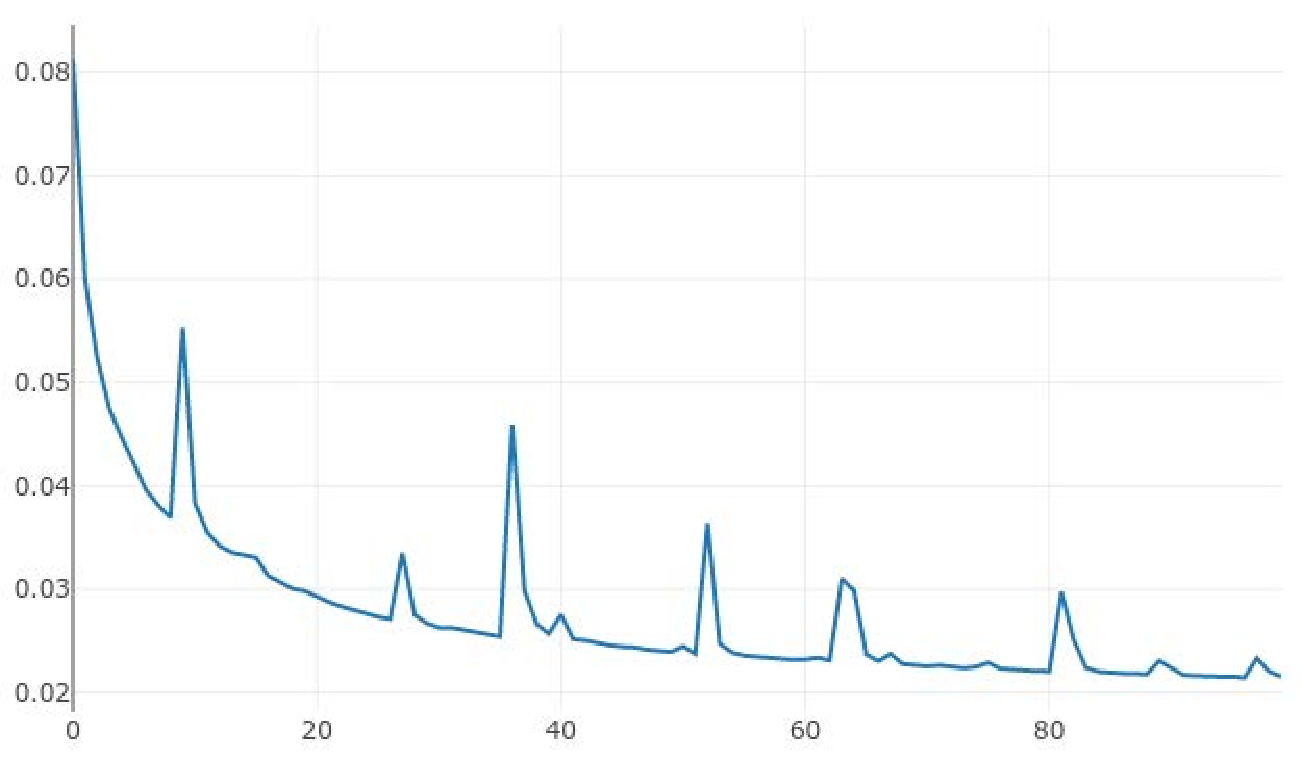
\includegraphics[width=0.5\textwidth]{fig16-a}\\
(a)\\[3ex]% add a little extra space
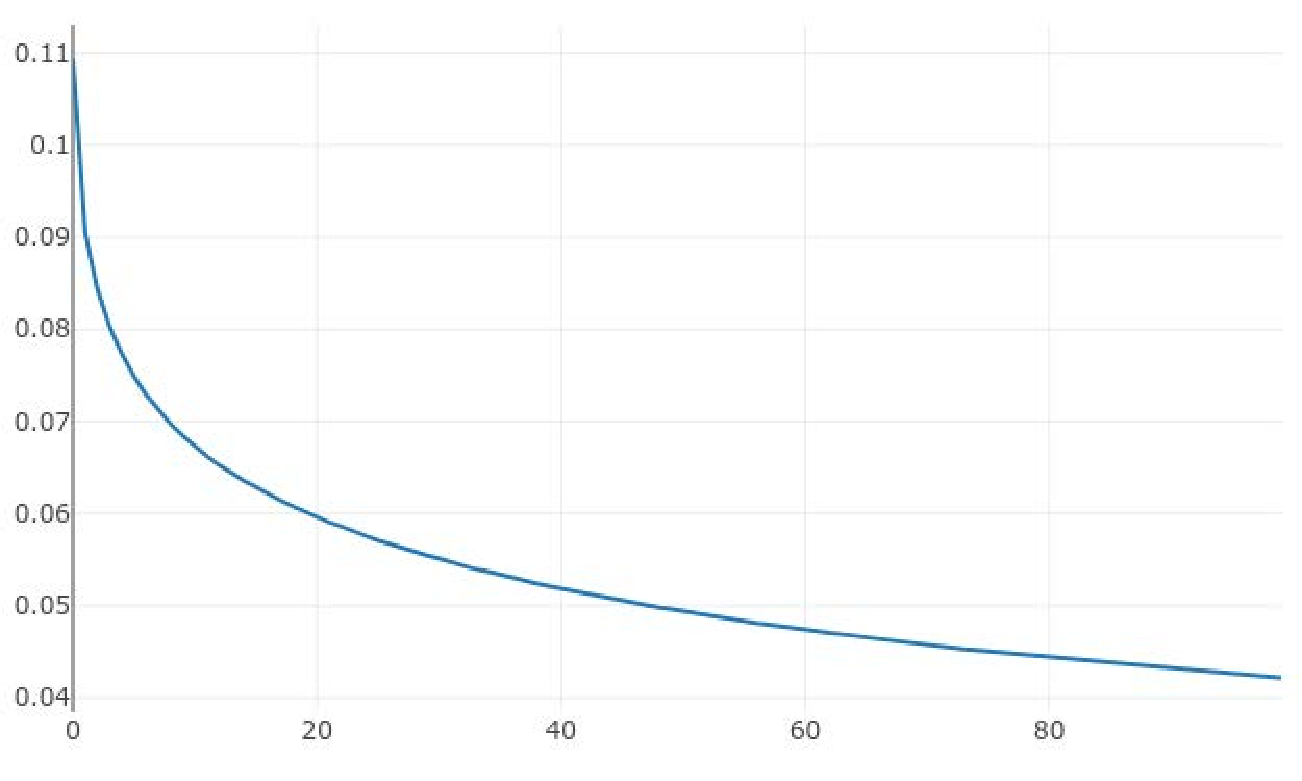
\includegraphics[width=0.5\textwidth]{fig16-b}\\
(b)\\[3ex]
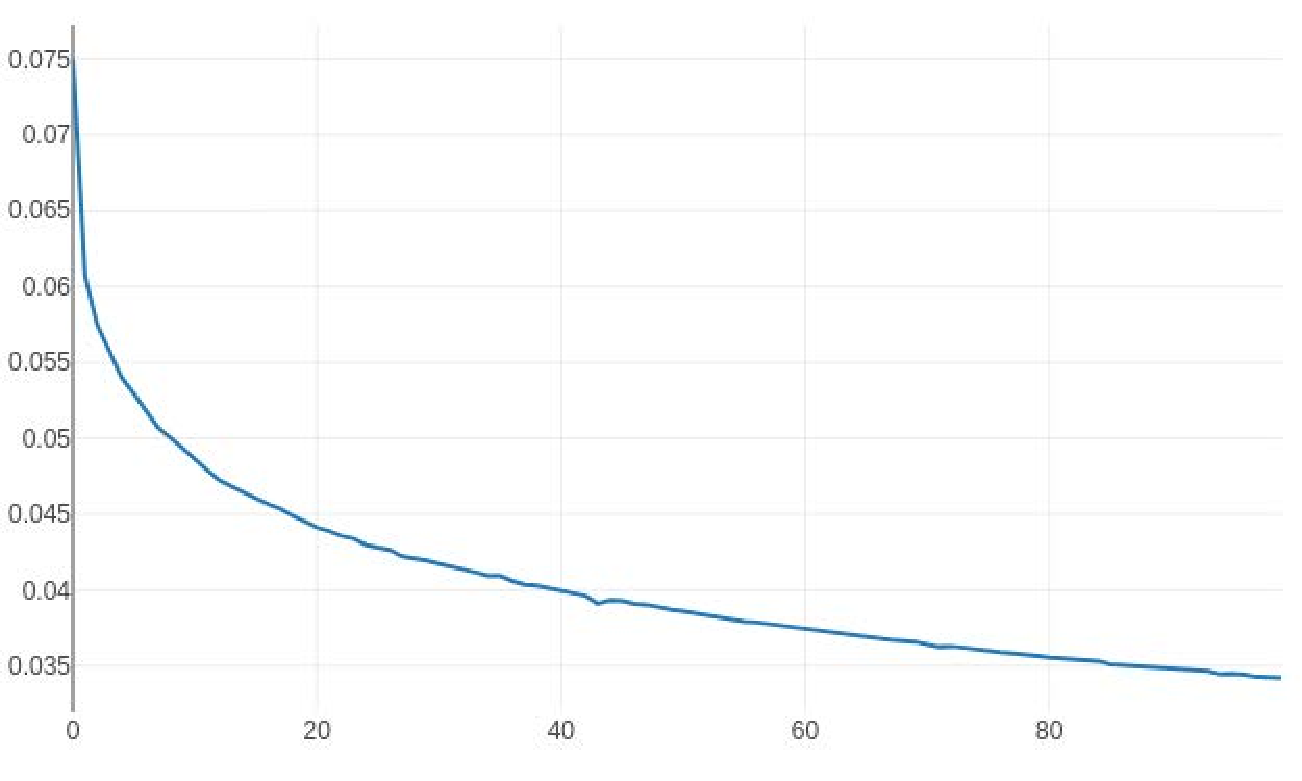
\includegraphics[width=0.5\textwidth]{fig16-c}\\
(c)
\end{tabular}
\caption{Epoch G loss. (a) Group 1, (b) Group 2, (c) Group 3.}%
\label{fig16}%
\end{figure}

\begin{figure}%
\centering\begin{tabular}{c}
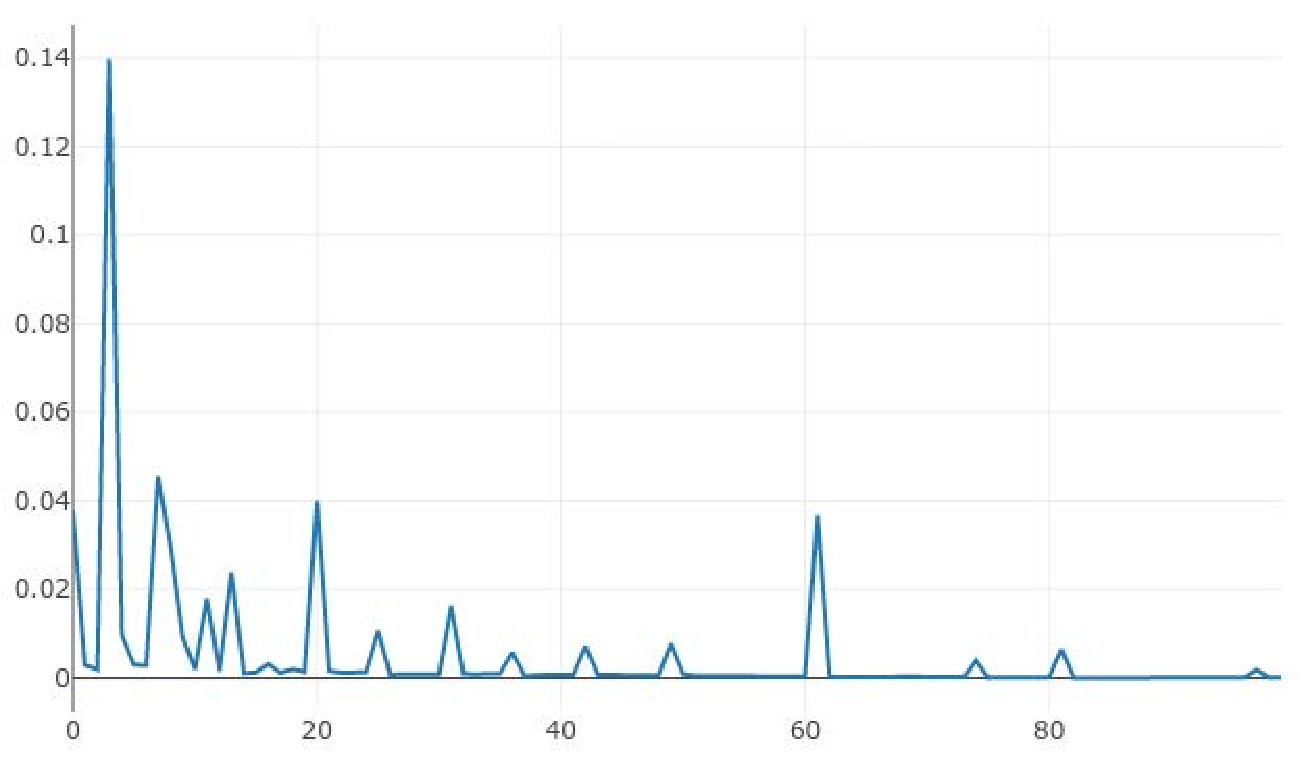
\includegraphics[width=0.5\textwidth]{fig17-a}\\
(a)\\[3ex]% add a little extra space
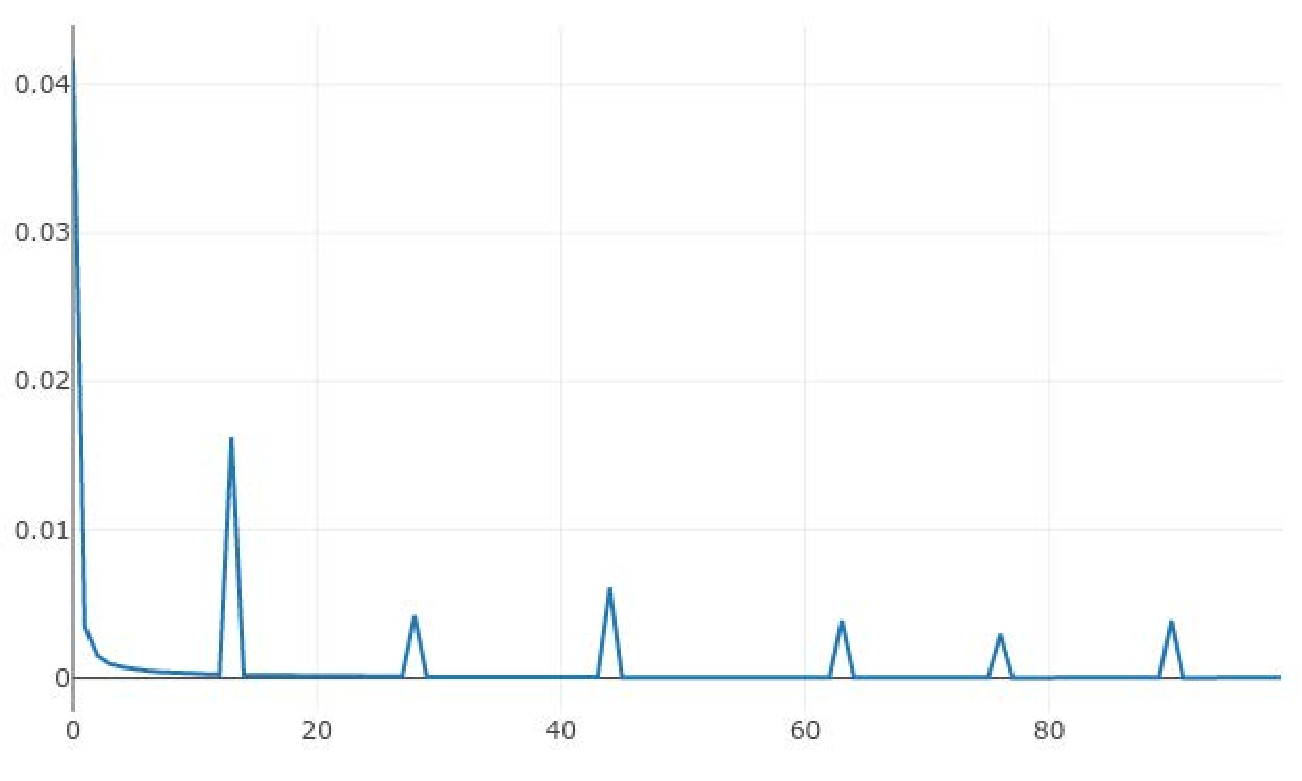
\includegraphics[width=0.5\textwidth]{fig17-b}\\
(b)\\[3ex]
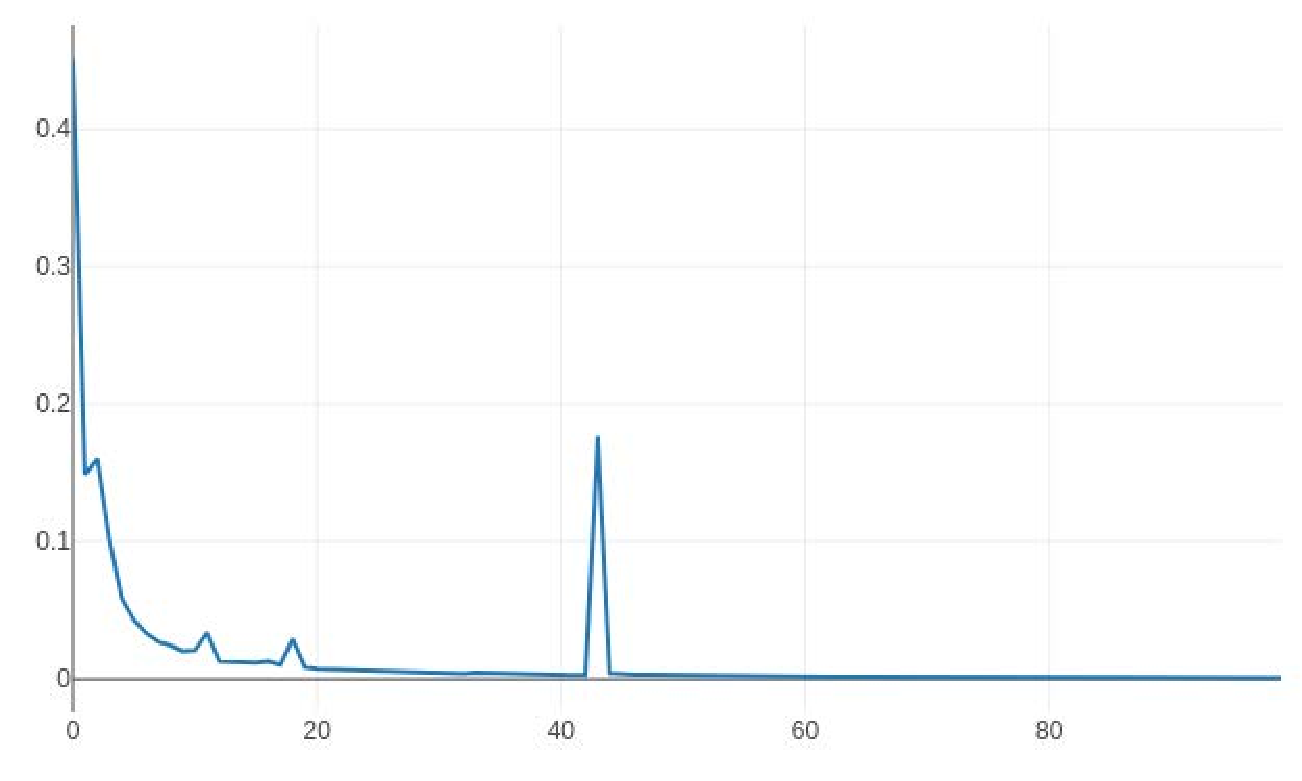
\includegraphics[width=0.5\textwidth]{fig17-c}\\
(c)
\end{tabular}
\caption{Epoch real loss. (a) Group 1, (b) Group 2, (c) Group 3.}%
\label{fig17}%
\end{figure}

\begin{figure}%
\centering\begin{tabular}{c}
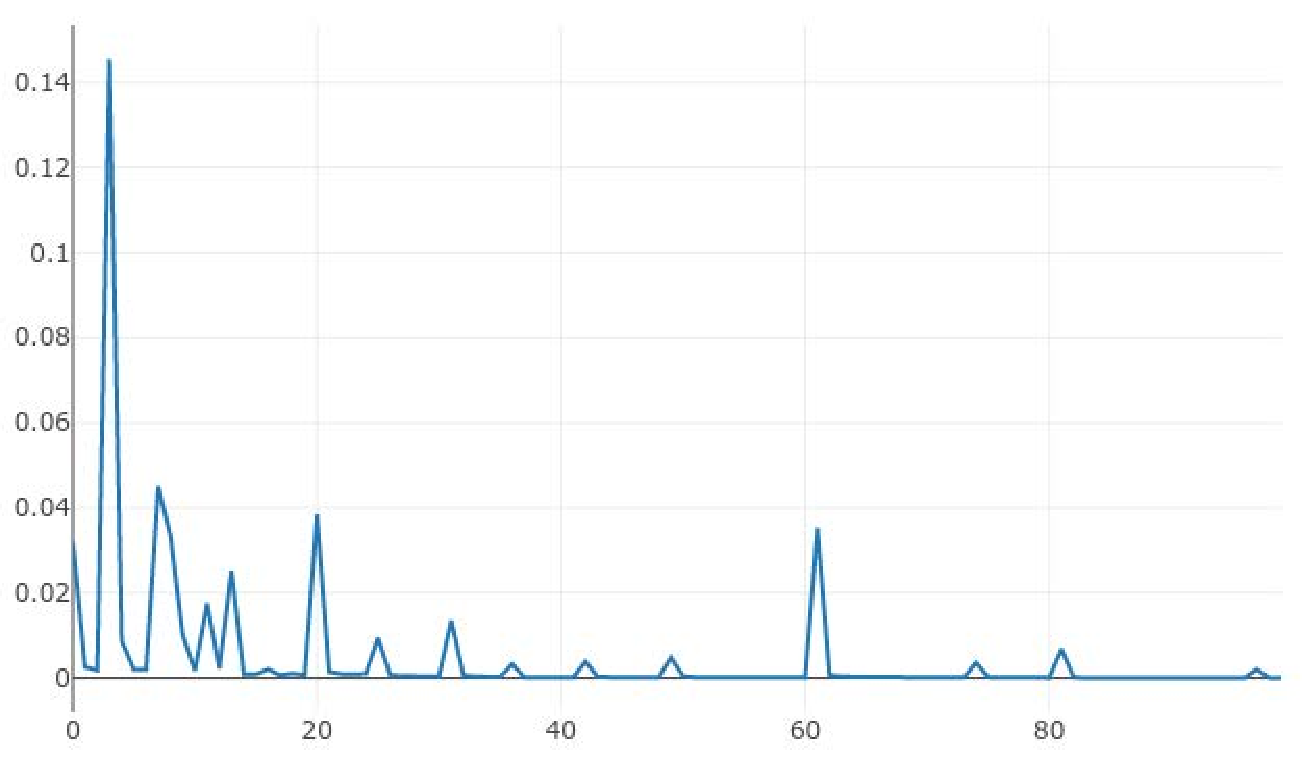
\includegraphics[width=0.5\textwidth]{fig18-a}\\
(a)\\[3ex]% add a little extra space
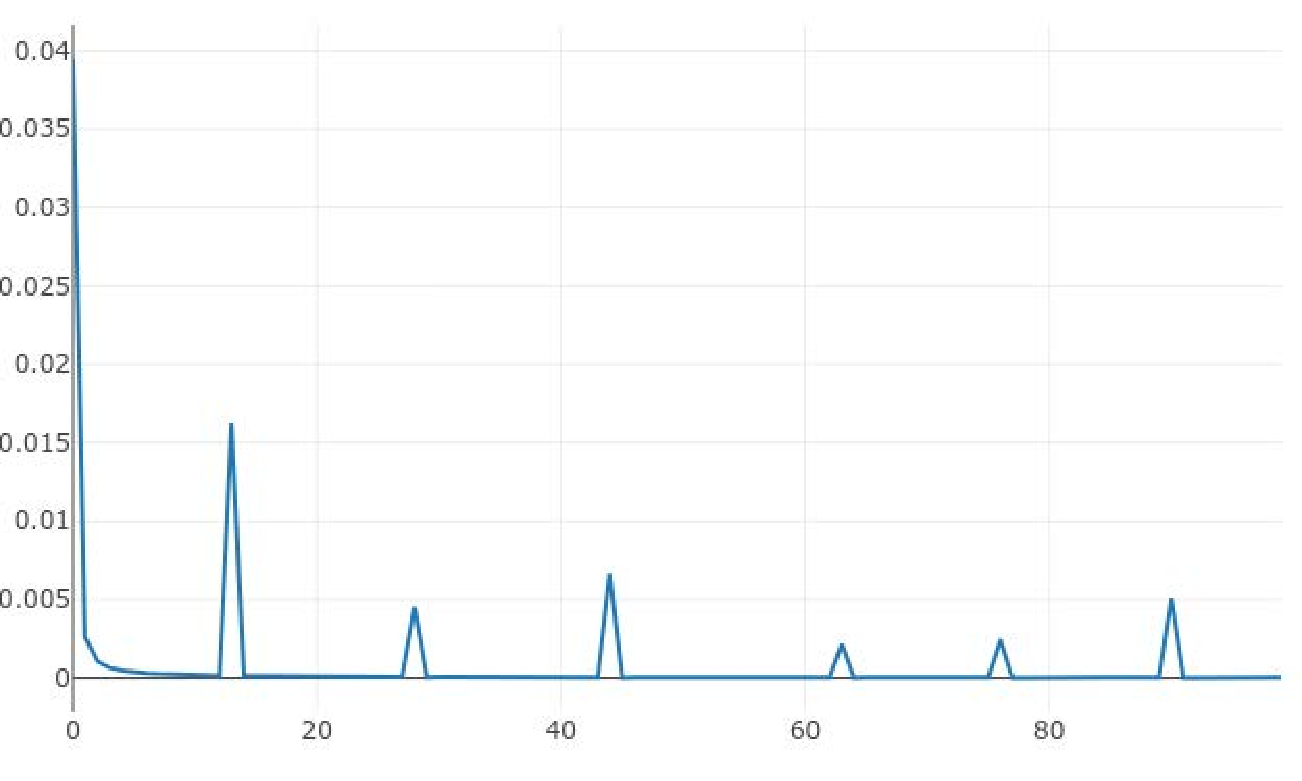
\includegraphics[width=0.5\textwidth]{fig18-b}\\
(b)\\[3ex]
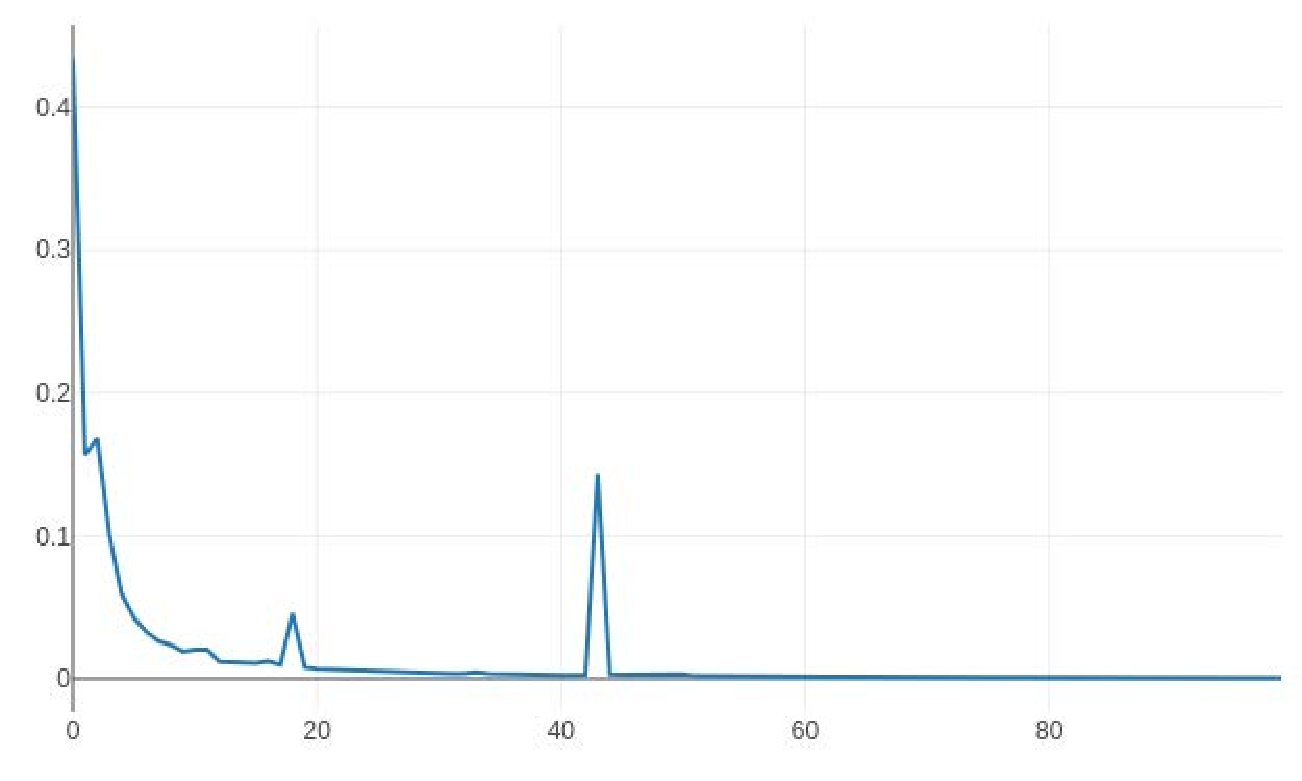
\includegraphics[width=0.5\textwidth]{fig18-c}\\
(c)
\end{tabular}
\caption{Epoch fake loss. (a) Group 1, (b) Group 2, (c) Group 3.}%
\label{fig18}%
\end{figure}

\begin{figure}%
\centering\begin{tabular}{c}
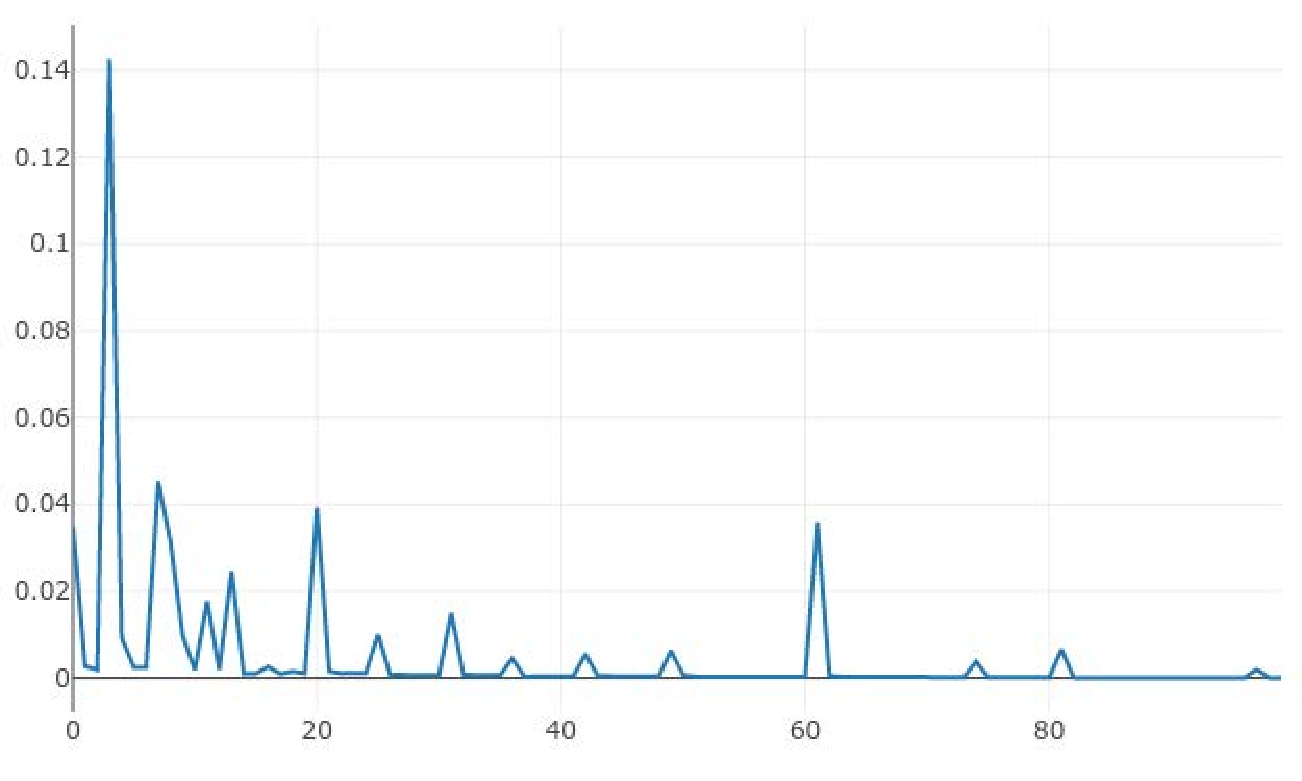
\includegraphics[width=0.5\textwidth]{fig19-a}\\
(a)\\[3ex]% add a little extra space
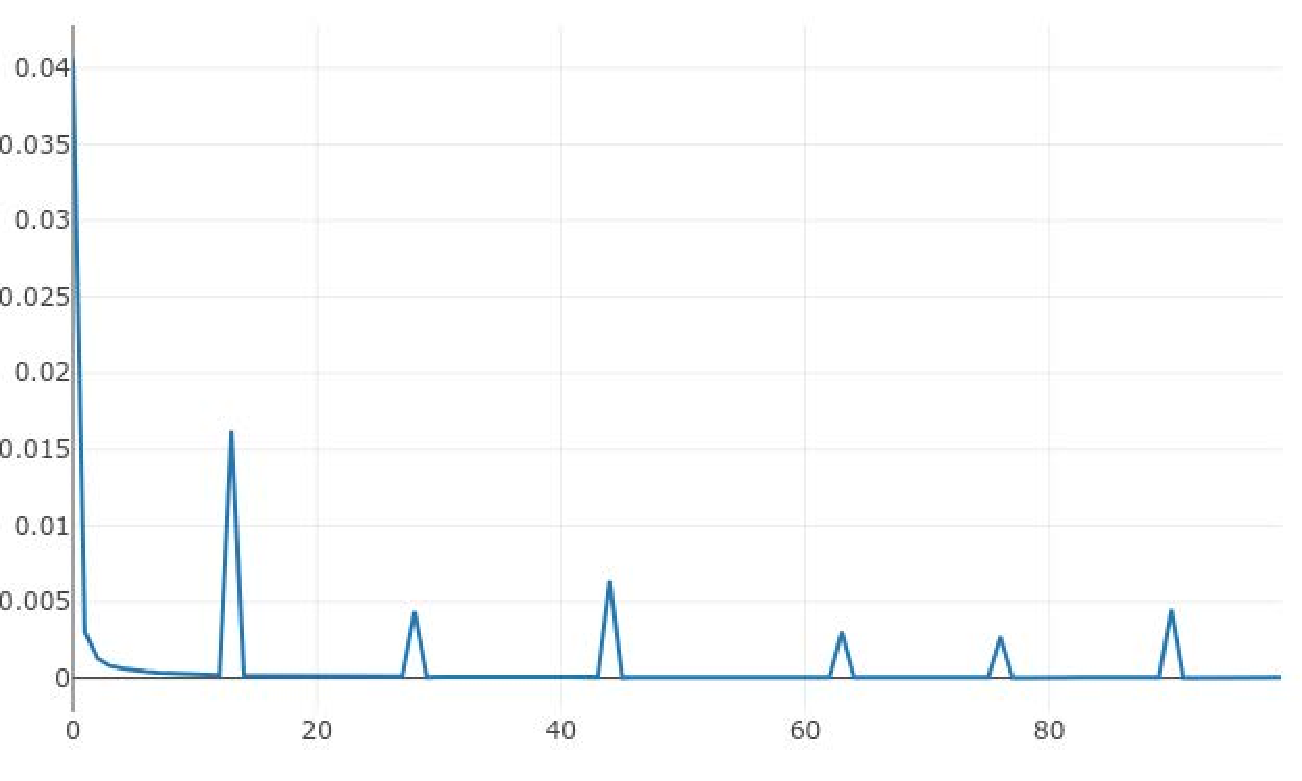
\includegraphics[width=0.5\textwidth]{fig19-b}\\
(b)\\[3ex]
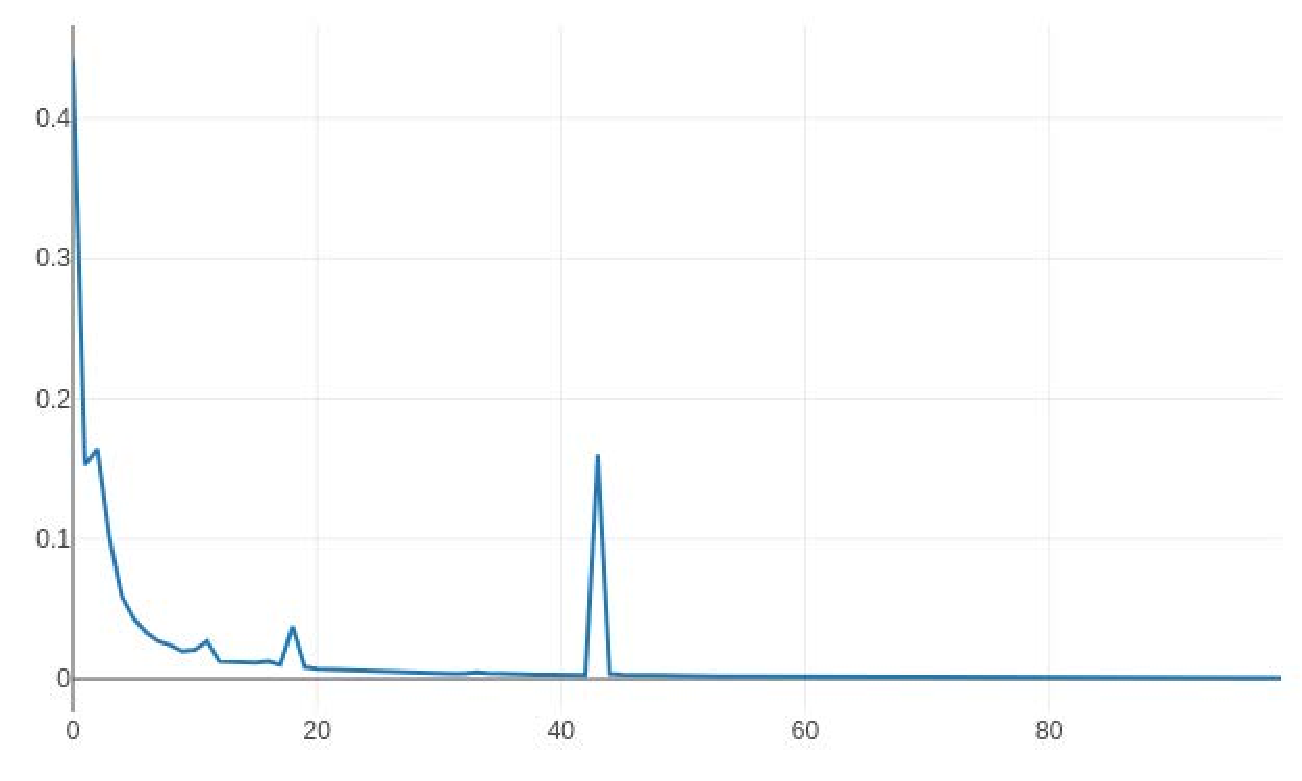
\includegraphics[width=0.5\textwidth]{fig19-c}\\
(c)
\end{tabular}
\caption{Epoch D loss. (a) Group 1, (b) Group 2, (c) Group 3.}%
\label{fig19}%
\end{figure}

\begin{figure}%
\centering\begin{tabular}{c}
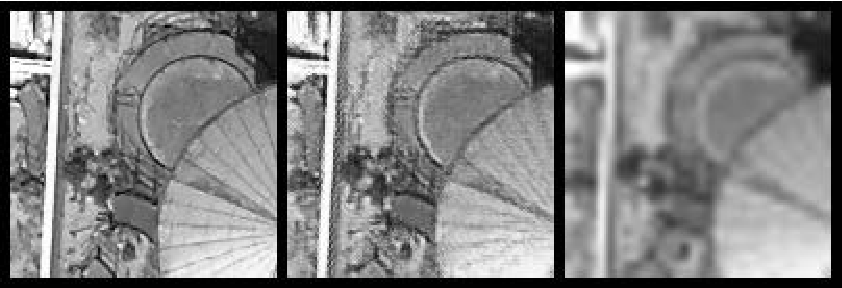
\includegraphics[width=0.5\textwidth]{fig20-a}\\
(a)\\[3ex]% add a little extra space
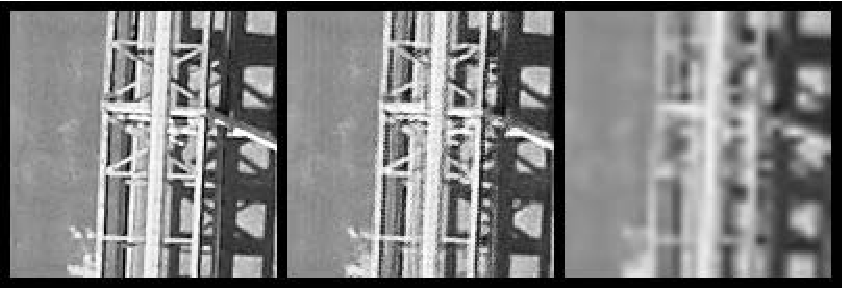
\includegraphics[width=0.5\textwidth]{fig20-b}\\
(b)\\[3ex]
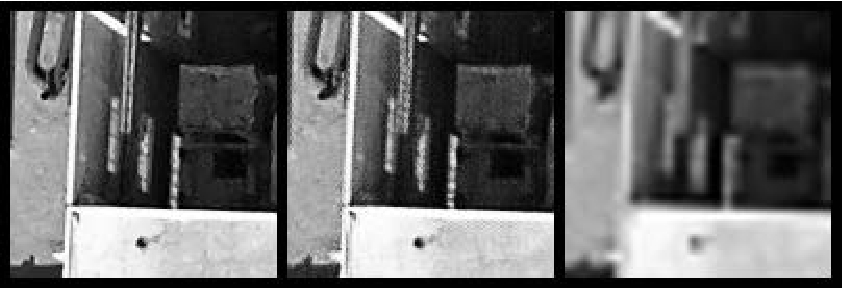
\includegraphics[width=0.5\textwidth]{fig20-c}\\
(c)
\end{tabular}
\caption{Reconstructed results by Group 1 (Ground truth, pbiSRGAN and Bicubic reconstruction are listed from left to right). (a) Oil tank, (b) Metal, (c) Roof.}%
\label{fig20}%
\end{figure}

\begin{figure}%
\centering\begin{tabular}{c}
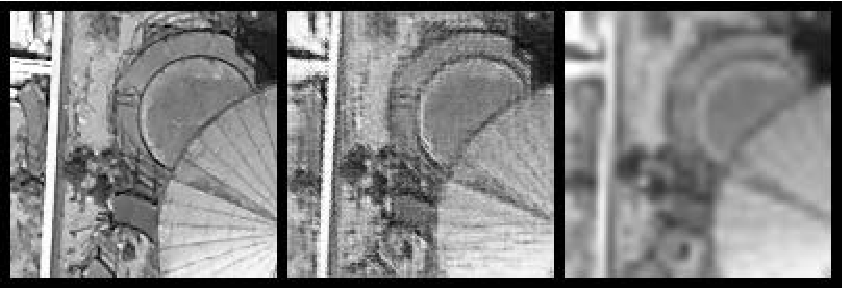
\includegraphics[width=0.5\textwidth]{fig21-a}\\
(a)\\[3ex]% add a little extra space
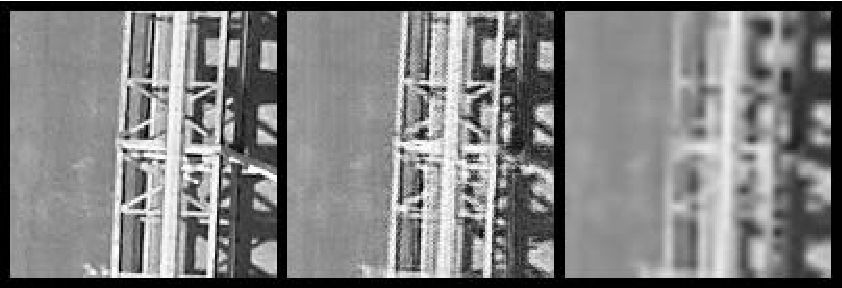
\includegraphics[width=0.5\textwidth]{fig21-b}\\
(b)\\[3ex]
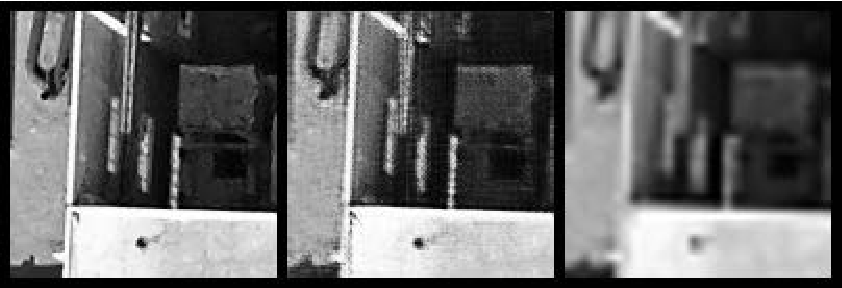
\includegraphics[width=0.5\textwidth]{fig21-c}\\
(c)
\end{tabular}
\caption{Reconstructed results by Group 2 (Ground truth, pbiSRGAN and Bicubic reconstruction are listed from left to right). (a) Oil tank, (b) Metal, (c) Roof.}%
\label{fig21}%
\end{figure}

\begin{figure}%
\centering\begin{tabular}{c}
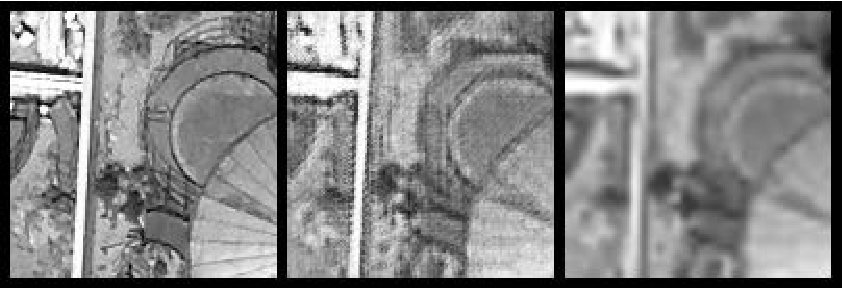
\includegraphics[width=0.5\textwidth]{fig22-a}\\
(a)\\[3ex]% add a little extra space
\includegraphics[width=0.5\textwidth]{fig22-b}\\
(b)\\[3ex]
\includegraphics[width=0.5\textwidth]{fig22-c}\\
(c)
\end{tabular}
\caption{Reconstructed results by Group 3 (Ground truth, pbiSRGAN and Bicubic reconstruction are listed from left to right). (a) Oil tank, (b) Metal, (c) Roof.}%
\label{fig22}%
\end{figure}

\begin{figure}%
\centering\begin{tabular}{c}
\includegraphics[width=0.5\textwidth]{fig23-a}\\
(a)\\[3ex]% add a little extra space
\includegraphics[width=0.5\textwidth]{fig23-b}\\
(b)\\[3ex]
\includegraphics[width=0.5\textwidth]{fig23-c}\\
(c)
\end{tabular}
\caption{Mean PSNR of reconstructed results from validation set. (a) Group 1, (b) Group 2, (c) Group 3.}%
\label{fig23}%
\end{figure}

\begin{figure}%
\centering\begin{tabular}{c}
\includegraphics[width=0.5\textwidth]{fig24-a}\\
(a)\\[3ex]% add a little extra space
\includegraphics[width=0.5\textwidth]{fig24-b}\\
(b)\\[3ex]
\includegraphics[width=0.5\textwidth]{fig24-c}\\
(c)
\end{tabular}
\caption{Mean SSIM of reconstructed results from validation set. (a) Group 1, (b) Group 2, (c) Group 3.}%
\label{fig24}%
\end{figure}


\begin{figure}%
\centering\begin{tabular}{c}
\includegraphics[width=0.5\textwidth]{fig25-a}\\
(a)\\% add a little extra space
\includegraphics[width=0.5\textwidth]{fig25-b}\\
(b)\\
\includegraphics[width=0.5\textwidth]{fig25-c}\\
(c)\\
\includegraphics[width=0.5\textwidth]{fig25-d}\\
(d)\\
\includegraphics[width=0.5\textwidth]{fig25-e}\\
(e)\\
\includegraphics[width=0.5\textwidth]{fig25-f}\\
(f)
\end{tabular}
\caption{Part of Reconstructed results on testing set (Ground truth, pbiSRGAN and Bicubic reconstruction are listed from left to right). (a) Reconstruction 1, (b) Reconstruction 2 ,(c) Reconstruction 3, (d) Reconstruction 4, (e) Reconstruction 5, (f) Reconstruction 6.}%
\label{fig25}%
\end{figure}


\begin{table}
\begin{center}
	\begin{tabular}{lccc}
		\hline		
		No.&Layer      &Input channel&Output channel\\
		\hline
		1  &Conv2d     &1        &64    \\
		2  &LeakyReLU  &-        &-       \\
		3  &Conv2d     &64       &64     	\\
		4  &BatchNorm2d&64       &64    \\
		5  &LeakyReLU  &-        &-        \\
		6  &Conv2d     &64       &128       \\
		7  &BatchNorm2d&128      &128      \\
		8  &LeakyReLU  &-        &-        \\
		9  &Conv2d     &128      &128     \\
		10 &BatchNorm2d&128      &128      \\
		11 &LeakyReLU  &-        &-      \\
		12 &Conv2d     &128      &256     \\
		13 &BatchNorm2d&256      &256 \\
		14 &LeakyReLU  &-        &-      \\
		15 &Conv2d     &256      &256     \\
		16 &BatchNorm2d&256      &256     \\
		17 &LeakyReLU  &-        &-       \\
		18 &Conv2d     &256      &512     \\
		19 &BatchNorm2d&512      &512     \\
		20 &LeakyReLU  &-        &-       \\
		21 &Conv2d     &512      &512     \\
		22 &BatchNorm2d&512      &512     \\
		23 &LeakyReLU  &-        &-       \\
		24 &Conv2d     &512      &1       \\
		\hline
	\end{tabular}
\end{center}
\caption{Parameters of discriminant network.}
\label{tab1}
\end{table}

\begin{table}
\begin{center}
	\begin{tabular}{lcc}
		\hline	
		No. &Parameters    &Value	\\
		\hline
		1  &Operating system &Linux Ubuntu18.04 \\
		2  &GPU model &Telsa K80\\
		3  &GPU memory &10GB\\
		4  &GPU number &3\\
		5  &CUDA version&10.2\\
		6  &CPU model  &Intel Xeon(R) \\
		7  &CPU memory &47GB\\
		8  &CPU clock speed &2.5GHz\\
		9  &CPU core number &12\\
		10 &CPU number &4\\
		\hline
	\end{tabular}
\end{center}
\caption{Hardware information for simulation.}
\label{tab2}
\end{table}

\begin{table}
\begin{center}
	\begin{tabular}{lccc}
		\hline	
		Hyperparameters		&Group 1      	 & Group 2		 &Group 3 \\
		\hline
		Traing epochs 			&100      	   &100    		&100 \\
		\makecell[l]{Training batch\\size}     	   &128       	  &128    	   &128\\
		\makecell[l]{Validation batch\\size}	   &1       	  &1      	   &1\\
		\makecell[l]{G learning rate}       &0.0002        &0.0002 	  &0.0002\\
		\makecell[l]{D learning rate}       &0.0002		 &0.0002 	  &0.0002\\
		\makecell[l]{Epoch of learning\\rate decay}		  &-         	&50      		&-\\
		\makecell[l]{Percentage of \\learning rate decay}   &-         	&$90\%$     &-\\
		Scaling factor          	&4             &4      	    &4      \\
		\makecell[l]{Training ratio\\of G and D}	&1:1	       &1:1    	    &5:1\\
		GPU number     	     &3             &3 			  &3      \\
		\makecell[l]{Height of\\HR images}	 &128           &128      	  &128    \\
		\makecell[l]{Width of \\HR images}	 	 &128        	&128          &128 \\
		\makecell[l]{Number of\\training images}     	   &96000     	  &96000 	    &96000  \\
		\makecell[l]{Number of\\validating images}   	   &3000          &3000        	&3000   \\
		\makecell[l]{Number of\\testing images}     		   &1000          &1000        	&1000   \\
		\hline
	\end{tabular}
\end{center}
\caption{Experimental scheme of pbiSRGAN}
\label{tab3}
\end{table}

\begin{table}
\begin{center}
	\begin{tabular}{lc}
		\hline	
		No. &loss	\\
		\hline
		1  &batch con loss \\
		2  &batch gen loss\\
		3  &batch G loss\\
		4  &batch real loss\\
		5  &batch fake loss\\
		6  &batch D loss \\
		7  &epoch con loss\\
		8  &epoch gen loss\\
		9  &epoch G loss \\
		10 &epoch real loss\\
		11 & epoch fake loss\\
		12 & epoch D loss \\
		\hline
	\end{tabular}
\end{center}
\caption{Two kinds of loss metrics: batch loss and epoch loss.}
\label{tab4}
\end{table}

\begin{table}
\begin{center}
	\begin{tabular}{lcccc}
		\hline	
		No. &Evaluation indicator & Group 1 & Group 2 & Group 3	\\
		\hline
		1  &PSNR  			&19.6652      	   &17.9452   		&16.4628 \\
		2  &SSIM     	   &0.6045       	  &0.5178    	   &0.4575\\
		\hline
	\end{tabular}
\end{center}
\caption{Mean PSNR and SSIM of reconstructed results from testing set.}
\label{tab5}
\end{table}

\end{document}
